\documentclass[./main_en.tex]{subfiles}
\graphicspath{{\subfix{./figs}}}

% ------------ main document ------------ 
\begin{document}

\chapter{\chapSysEn} \label{chap:systems}

% custom paragraph skip
\setlength{\parskip}{0mm}

\epigraph{\small{Everything we think we know about the world is a \gls{model}. Every word and every language is a \gls{model}. All maps and statistics, books and databases, equations and codes are models. So are the ways I imagine the world in my head -- my \gls{mental-models}. None of these is or ever will be the real world.}}{Donella Meadows (2008, p. 86) \cite{meadows2008}}

\epigraph{\small{If validation is impossible and all models are wrong, why do we bother to build them? As a leader, you must recognize that you will be using a \gls{model} -- mental or formal -- to make decisions. Your choice is never whether to use a \gls{model}, but which \gls{model} to use. Your responsibility is to use the best \gls{model} available for the purpose at hand, despite its limitations. Delaying actions in the vain search for a perfect \gls{model} is, in itself, a decision, with its own consequences.}}{John Sterman (2000, p. 850) \cite{sterman2000}}


% custom paragraph skip
\setlength{\parskip}{\myparskip}

\section{The Modeling Process} \label{sec:sys:process}

\par Donella Meadows (1941-2001) may have been the most brilliant environmental systems modeler to ever live, leading the ambitious initiative proposed by the book \textit{Limits to Growth}, published in 1972 and revised in two subsequent editions. This book issued an unprecedented warning about the ecological scenarios that the current industrial society, based on non-renewable resources, may face by the year 2100, including the possibility of a catastrophic collapse \cite{meadows1974}. Her argumentation was based on simulations of a comprehensive \gls{model} of the world, the \gls{model} \texttt{World3}, mapping the availability of numerous stocks and flows of natural resource consumption, from arable land to oil reserves. Despite the significant social, political, and economic impact of her work, Meadows contributed little toward the more philosophical direction, such as the epistemological problems addressed in Chapter 1. Still, as emphasized in the above epigraph, she left evidence of sharing the Kantian tradition, according to which pure reason has access only to transcendent categories or, in her terms, to \textbf{\gls{mental-models}}. These \gls{mental-models} would then be expressed in various forms, including diagrams, texts, equations, and computer programs. Her line of thought eventually suggests an instrumentalist view, in which we will never have the conditions to establish the truth about the world, but only empirically adequate theories:

% figure
\begin{figure}[t!] % place figure in the page
	\centering				
	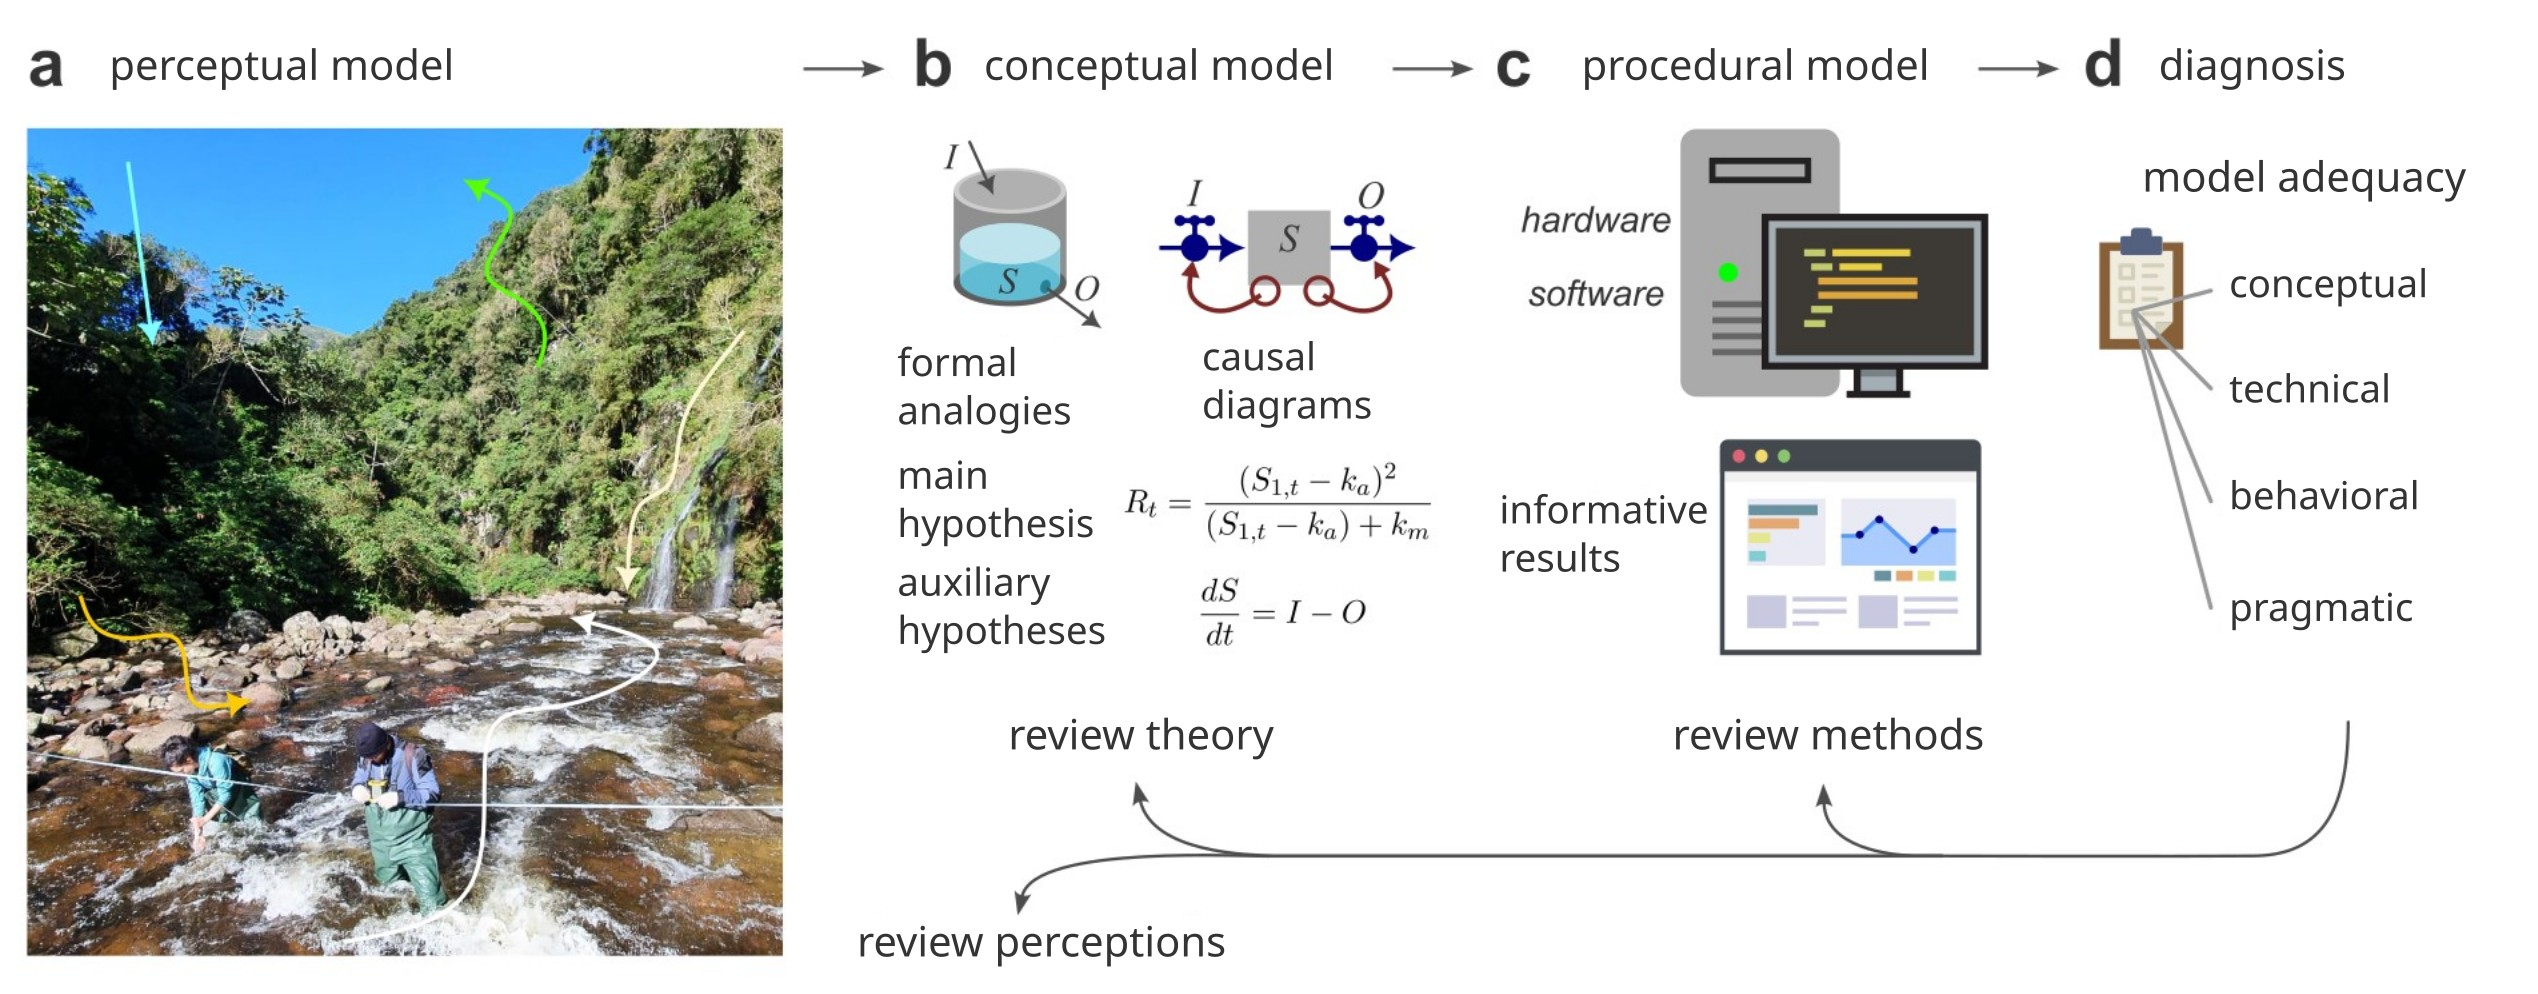
\includegraphics[width=0.95\linewidth]{figs/fig_modelprocess_en.jpg}		
	\caption[The Modeling Process]
	{\textbf{---\;The modeling process.}
        Hydrological modeling can be understood as an iterative learning process. \;\textbf{a}\;---\;The first stage consists of the \gls{percept-model} (\gls{mental-models}), which is a collection of subjective and personal perceptions acquired through empirical experience (field expeditions) and theoretical experience (textbooks, lectures, classes, etc). \;\textbf{b}\;---\;The second stage consists of the \gls{concept-model}, which instantiates formal (mathematical) analogies and causal diagrams (structures) to obtain an objective main \gls{hipotese} in the form of equations. Various \gls{aux-hyp} are generally required, making the \gls{concept-model} a logically open \gls{system} (underdetermined). \;\textbf{c}\;---\;The third stage consists of the \gls{proced-model}, which is the synthesis of the computational methods used (\textit{hardware} and \textit{software}) to simulate the \gls{concept-model} and produce results in symbolic forms such as tables, graphs, maps, animations, etc. \;\textbf{d}\;---\;Finally, the diagnostic stage applies various procedures to assess the adequacy of the models in conceptual (theoretical problems), technical (computational problems), behavioral (empirical justification), and practical (decision-making impacts) terms. The diagnosis is iterative, reviewing all created models and closing the learning cycle. The photograph in (\textbf{a}) was kindly provided by hydrologist Marina Fagundes, who is measuring the flow of a mountain river during a field expedition in Rio Grande do Sul, Brazil.\;
	}
\label{fig:sys:process}  % use qualitative label			
\end{figure}

\begin{adjustwidth}{100pt}{0pt}
\medskip
\small Our models usually have a strong congruence with the world. That is why we are such a successful species in the biosphere. Especially complex and sophisticated are the mental models we develop from direct, intimate experience of nature, people, and organizations immediately around us. However, and conversely, our models fall far short of representing the world fully. That is why we make mistakes and why we are regularly surprised. In our heads, we can keep track of only a few variables at one time. We often draw illogical conclusions from accurate assumptions, or logical conclusions from inaccurate assumptions. -- Donella Meadows \cite{meadows2008}.
\medskip
\end{adjustwidth}

\noindent Regardless of Meadows' position on philosophical currents, her view is clear in that modeling is a \textit{process} that begins in a \textit{subjective and personal} manner with \gls{mental-models}, and then becomes increasingly \textit{objective and impersonal} through texts, equations, and computer programs.

\par In the field of \gls{hydrology}, Keith Beven emphasizes Meadows' perspective, proposing that the modeling process consists of at least three stages represented by models of different natures: the \textit{perceptual} stage, the \textit{conceptual} stage, and the \textit{procedural} stage\footnote{Two additional stages in the modeling process include the calibration and validation of the \gls{proced-model}, but these stages are not models themselves; rather, they are steps of empirical justification.} \cite{beven2011}. Figure \ref{fig:sys:process} illustrates this conception, including a final diagnostic stage. The \textbf{\gls{percept-model}} begins with the hydrologist's subjective and qualitative understanding of how a watershed responds to precipitation events. This \gls{model} is profoundly influenced by individual experiences, studies, analyzed data, and the hydrologist's field experience. It is an inherently personal \gls{model} and varies substantially from person to person. Moving to the \textbf{\gls{concept-model}}, Beven describes a transition to a more formalized and simplified representation of the processes identified in the \gls{percept-model}. This \gls{model} involves creating hypotheses and adopting assumptions to \textit{abstract} the complex processes of reality into tangible and objective forms, often utilizing mathematical formulations. Finally, the \textbf{\gls{proced-model}} represents the practical implementation of the \gls{concept-model} in a computer program. At this stage, the equations and concepts from the \gls{concept-model} are translated into code, allowing simulations and predictions of flows and levels based on \gls{input-data} through the application of tensions in electronic circuits. In the case of digital computers, this process involves the application of numerical methods and may introduce additional errors or approximations, making precision and care in execution extremely important. It is these electronic computations that produce the supposedly informative results we see in tables, graphs, maps, etc. For Beven, the interaction and evolution between these three models are crucial in the modeling process in \gls{hydrology}. With several caveats, he includes two additional stages, which would be the \textit{calibration} and \textit{validation} of the \gls{model} against empirical evidence. These are jargons of \gls{prag-realism}. An instrumentalist nomenclature would be \textit{conditioning} and \textit{testing} against empirical evidence. One way or another, a final stage of \textbf{diagnosis} should lead to the review and refinement of the previously developed models, giving rise to an \textit{iterative learning cycle} and potential \textit{scientific revolutions} in understanding hydrological processes.

\par It is with this perspective that the objective of this chapter is to establish the necessary details about the modeling process so that we can soon discuss hydrological models properly. At a certain point in the previous chapter, it became essential to define a \gls{model} as a \textbf{symbolic vehicle of a theory}, a typically instrumentalist conception that resonates with Nancy Cartwright's view \sethlcolor{pink}\hl{[todo:cite]} -- which is effective in articulating the epistemological problems that underlie modeling practices. In this perspective, models are seen as mere translators of our theories or hypotheses about real phenomena, such as the \gls{hydro_cicle}. However, this is still a generic and abstract definition that does not provide a concrete understanding of the exact nature of models. As emphasized at the beginning of the first chapter, hydrological models materialize in the states of electronic circuits in digital computers, but they are also other things before this materialization. To articulate the enigma of what exactly models are, this chapter will abandon the domain of Epistemology and the Philosophy of Science, delving into the field of Ontology of models. I will address the problem of representation, the \gls{paradigma} of systems, \gls{sys-dyn}, and \gls{model-diags}. If in the previous chapter we were on a panoramic view with thin air, like at the top of a mountain, we are now certainly descending from the heights, following the valleys of the streams. The \gls{analogy} remains interesting, as the path is still difficult and steep, but the landscape is becoming increasingly familiar. Hope grows that soon we will be on gentle and open ground.

\section{Representation} \label{sec:sys:represent}

\par Models serve the function of representing a \textbf{\gls{sys-target}}. That is, precisely because they symbolically convey a \gls{teoria}, models aim to re-interpret a given phenomenon or entity that supposedly exists and develops in the real world. The problem of justifying the correspondence between the \gls{model} and reality was the subject of the first chapter. Here, however, we have a new problem: \textit{how is it possible to create the representations themselves}? The solution to this \textbf{\gls{problem-repr}} consists of establishing a process of \textbf{\gls{idealization}} of the \gls{sys-target} combined with the application of \textbf{\gls{infer-analog}}, that is, the construction of a \textbf{\gls{analogy}} between the \gls{sys-target} and the \gls{model}. In this line, Mary Hesse proposes that such analogies manifest both through \textit{material models}, semantic structures realized by physical objects, and through \textit{formal models}, syntactic structures expressed by mathematical equations implemented by computer programs \cite{hesse2017}.

\par The process of \gls{idealization} is the foundation of all modeling and is characterized by \textit{deliberate simplifications}, which make the \gls{model} more tangible and understandable than the \gls{sys-target} itself, emphasizing crucial aspects while ignoring supposedly less relevant details. According to R. Frigg and S. Hartmann \cite{sep-models-science}, there are two forms of \gls{idealization} that are not mutually exclusive: \textbf{\gls{idealiz-arist}} and \textbf{\gls{idealiz-galil}}. In the case of \gls{idealiz-arist}, the key lies in the process of \textbf{\gls{abstraction}}, when all supposed superficialities of the \gls{sys-target} are removed, leaving only a supposed \textit{essence}. In other words, \gls{abstraction} aims to preserve the truth, albeit only the part that is relevant. In a hydrological \gls{model}, for example, the vegetation canopy is usually treated as a single reservoir that intercepts rainwater. It is clear that each leaf and twig plays a role in \gls{interception}, but this individual process is considered irrelevant and abstracted as a general process occurring throughout the canopy. Alan Musgrave, however, notes that \gls{abstraction} can also result in falsehoods, especially when \textbf{\gls{neglig-premis}} are introduced, that is, when a \textit{knowingly true} causal factor is neglected \cite{musgrave1981}. He initially brings this critique to neoclassical economic theories, but it is also the case, for instance, when hydrological models ignore the importance of solar radiation and terrain shading on evaporative processes. The \gls{idealiz-galil}, on the other hand, consists of applying a controlled experimental distortion, which can be incrementally reversed from the simple to the complex, from the ideal to the real \cite{MCMULLIN1985}. In other words, \gls{idealization} exhibits an \textit{asymptotic behavior} that, in the limit, makes the \gls{model} identical to the \gls{sys-target}. The reference to Galileo Galilei (1564-1642) relates to his famous experiments with inclined planes, which led him to conclude that objects fall at the same time, regardless of their mass. In this case, the inclined plane idealized free fall, allowing for a better understanding of the physical process. In hydrological models, an example of this type of \gls{idealization} is the spatial discretization into response units, sub-basins, or drainage networks – when taken to the extreme of small parcels, it asymptotically approaches the watershed.

% figure
\begin{figure}[t!] % place figure in the page
	\centering				
	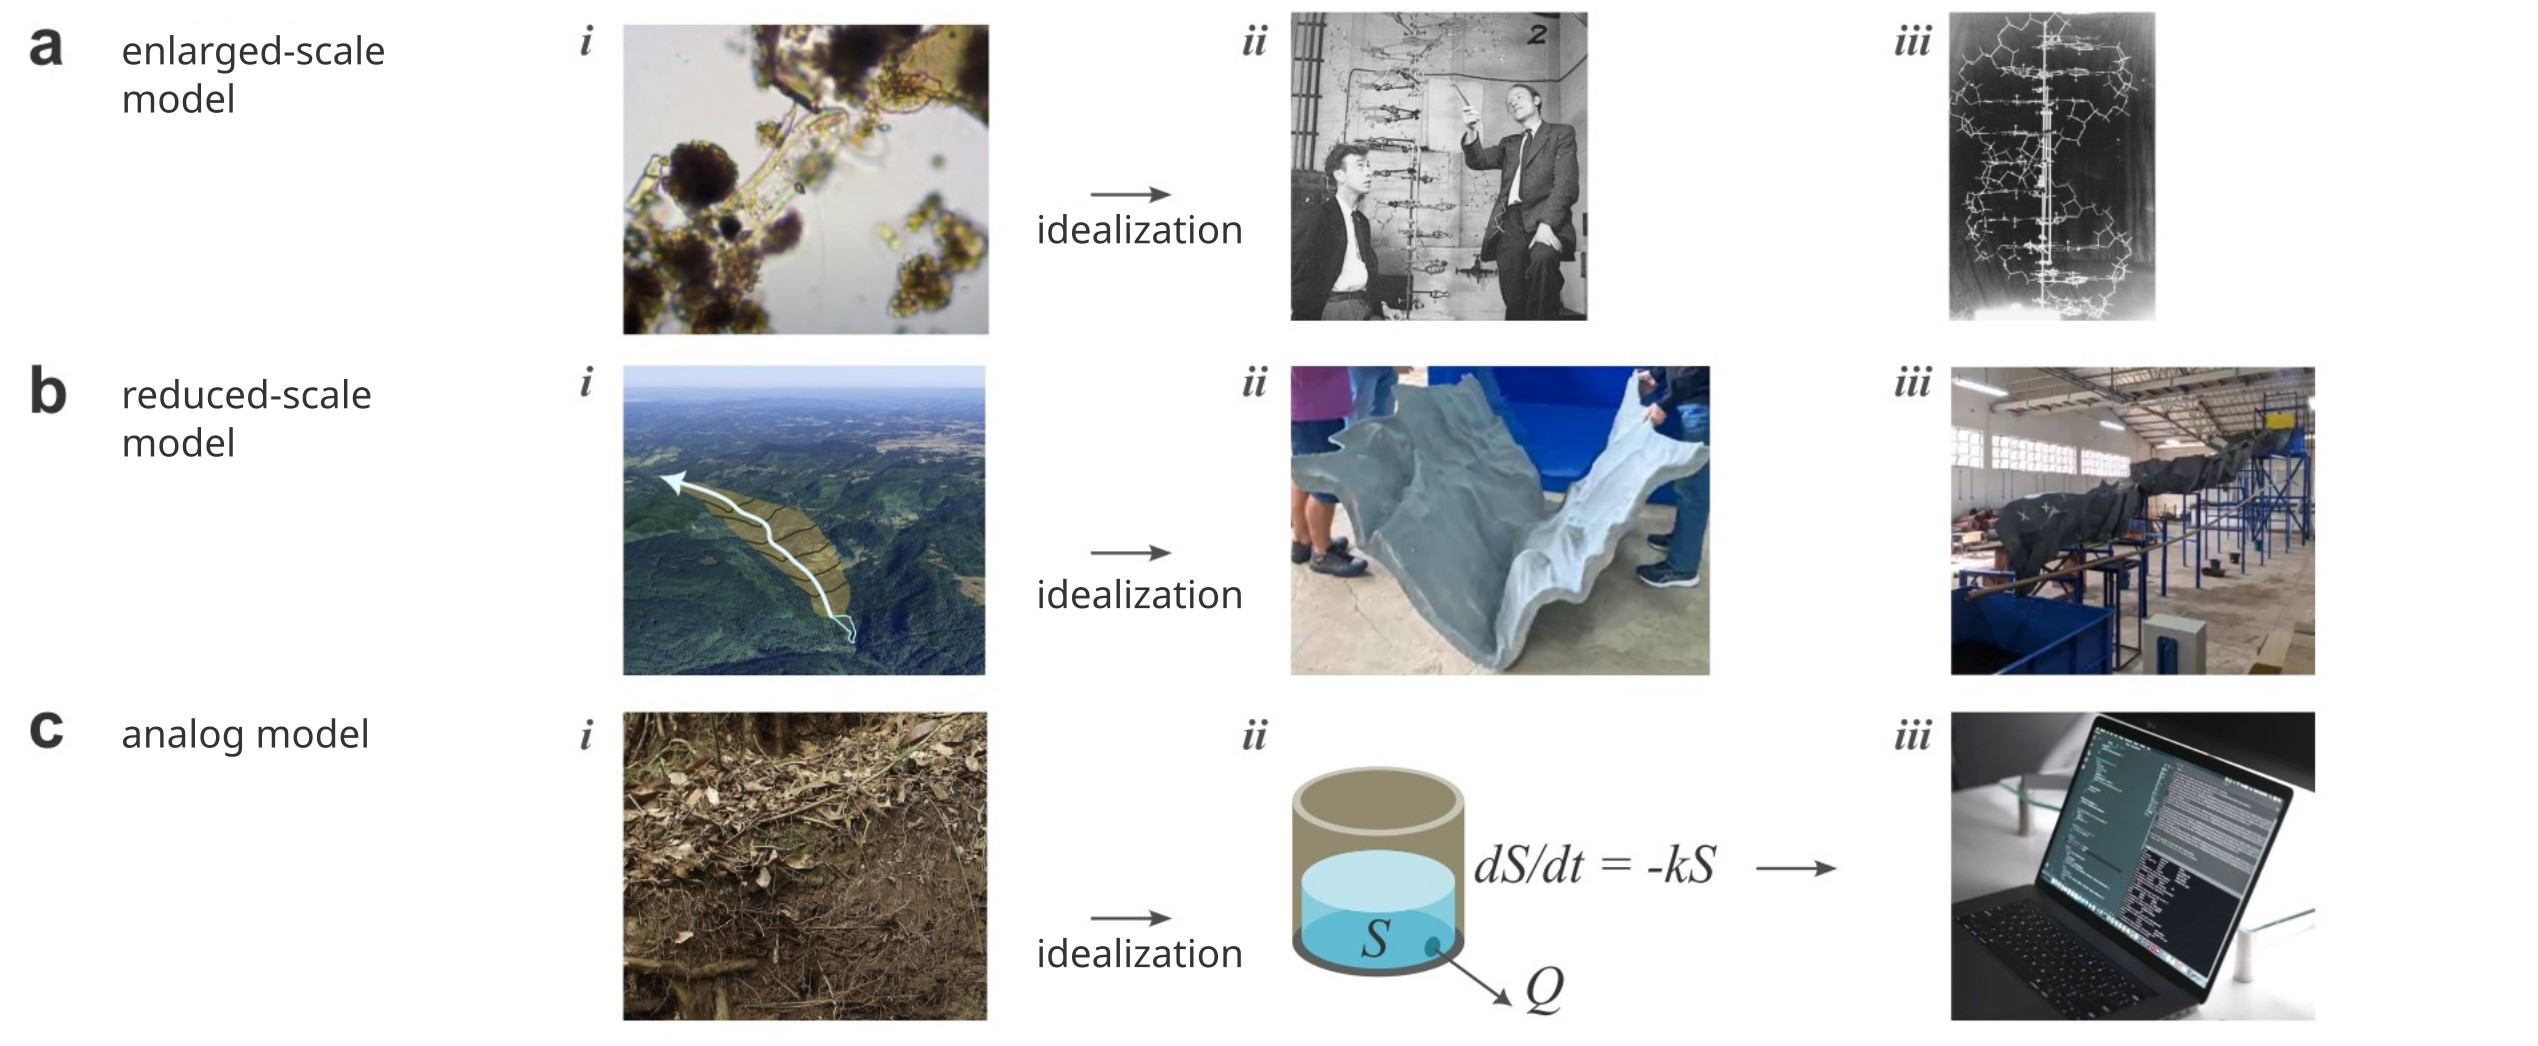
\includegraphics[width=0.95\linewidth]{figs/fig_representation_en.jpg}		
	\caption[Representation of systems by models]
	{\textbf{---\;Representation of systems by models.}
        \gls{idealization} is necessary to represent target systems in sufficiently tractable models.\;\textbf{a}\;---\;A famous enlarged-scale \gls{model} in the History of Science was the double helix \gls{model} for the DNA molecule, which stores the genetic code of organic cells (detail \textrm{\textit{i}}); Francis Crick and James Watson handling the \gls{model} (detail \textrm{\textit{ii}}); the original DNA \gls{model} (detail \textrm{\textit{iii}}).\;\textbf{b}\;---\;A reduced-scale \gls{model} for empirical studies of dam breakage. In this case, the \gls{model} represents 5.5 km of the valley downstream from the Canastra dam, Canela, Rio Grande do Sul (detail \textrm{\textit{i}}); the topobathymetric representation of the valley (detail \textrm{\textit{iii}}) with cross-section modules and steel long beams, filled with fiberglass and resin (detail \textrm{\textit{ii}}).\;\textbf{c}\;---\;A typical analog \gls{model} of \gls{hydrology} for water storage in the soil and groundwater (detail \textrm{\textit{i}}); the formal \gls{analogy} (homology) is made with a \gls{linear-reserv}, as if it were a bucket with a porous outlet at the bottom (detail \textrm{\textit{iii}}); the \gls{model} is realized in a digital computer, from the interaction of \textit{hardware} with \textit{software} (detail \textrm{\textit{iii}}).\;Credits for the images: (\textbf{a}) the author (detail \textrm{\textit{i}}) and from Chadarevian \cite{deChadarevian2003} (details \textrm{\textit{ii}} and \textrm{\textit{iii}}); (\textbf{b}) the author (detail \textrm{\textit{i}}) and Flávia Pereira \cite{Pereira2023} (details \textrm{\textit{ii}} and \textrm{\textit{iii}}); (\textbf{c}) the author (detail \textrm{\textit{i}}) and Pinterest (detail \textrm{\textit{iii}}).
	}
\label{fig:sys:represen}  % use qualitative label			
\end{figure}

\par Among the available forms of analogies, a somewhat direct alternative is to construct a \textit{copy} of what is understood as the \gls{sys-target}, at a scale suitable for manipulation by humans. These material models are referred to as \textbf{\gls{scale-models}} reduced or enlarged, illustrated in Figure \ref{fig:sys:represen}a and Figure \ref{fig:sys:represen}b. To some extent, we are all accustomed to models of this type, as the toys we played with as children are like reduced-scale models. A scale model of a building or a car in a wind tunnel, for example, is a reduced-scale \gls{model} used for engineering applications. Atoms of chemical elements with fittings to form more complex molecules, on the other hand, are enlarged-scale models for educational purposes. In a highly technological age, \gls{scale-models} may seem crude or simplistic, but they are actually extremely interesting options for investigating, visualizing, and experimentally testing the implications of a given \gls{teoria} or \gls{hipotese}. A notable example in the History of Science that involved the contribution of an enlarged-scale \gls{model} was the discovery of the structure of DNA by Watson and Crick in the early 1950s \cite{deChadarevian2003}. Despite their appeal, the \textbf{\gls{scale-similarity}} of representation is only feasible in special cases or for certain characteristics. For example, if a model of a city is built to observe the shading effects of buildings, the reduction of scale does not interfere with the shadow patterns produced by light, as the geometry is completely preserved at both scales. However, a reduced-scale water channel or pipe may exhibit viscosity and surface tension effects much greater than those observed at the real scale, making the conversion between scales a non-trivial problem. In fluid mechanics problems like this, the conversion is usually solved through dimensional analysis, which seeks to establish a characterization of the \gls{sys-target} that is scale-free, such as the Mach, Reynolds, and Froude numbers.

\par Depending on the \gls{sys-target} in question, representation by reduced or enlarged \gls{scale-models} may not be possible due to some fundamental principle or simply due to a lack of material resources. An epidemiological \gls{model} at a reduced scale is clearly not possible for ethical reasons, for example. Meanwhile, a reduced-scale \gls{model} of an environmental \gls{system}, such as a floodplain or the atmosphere itself, can be very expensive. Given this condition, it is necessary to resort to a form of analogical representation. In other words, it is essential to adopt a modeling approach that establishes a formal \gls{analogy}, or \textbf{\gls{homology}}, with the \gls{sys-target}, that is, an equivalence between the \textit{mathematical structures} of the \gls{sys-target} and the \gls{model}. In \gls{hydrology}, this is often achieved by establishing that the soil (or any other compartment of the hydrological cycle) functions \textit{as if} it were a \gls{linear-reserv}, like a bucket with a porous hole at the bottom, as illustrated in Figure \ref{fig:sys:represen}c. The conjunctive phrase \say{as if} is crucial, as it establishes the \gls{analogy} that underpins the \gls{idealization} of modeling. The implementation of the formal \gls{analogy}, that is, the realization of its mathematical structure, generally occurs through the programming of digital computers (which is the case for hydrological models), although it is also possible to create material models of the analogous \gls{system}. In this sense, formal models make the symbolic conveyance of the \gls{teoria} or \gls{hipotese} about the \gls{sys-target} much clearer than \gls{scale-models}, as they seek to test a mathematical structure based on a supposedly analogous \gls{system}. Just like deduction, induction, and abduction mentioned in the \gls{contexto-justificacao} of theories in the first chapter, the \gls{analogy} also constitutes a form of inference, which presents the following logical structure \cite{shaw_ashley_1983}:
\begin{enumerate}
    \item The objects $O_1, O_2, O_3, ... O_n$ share the properties $P_2, P_3, P_4, ... P_k$. 
    \item The objects $O_2, O_3, ... O_n$ share the property $P_1$. \\
    \item Therefore, it is likely that the object $O_1$ possesses the property $P_1$.
\end{enumerate}
Thus, \gls{infer-analog} allows for multiple items to be evaluated, although generally the relationship is made between only two objects – in the case of modeling, the \gls{sys-target} and the \gls{model}. Another characteristic is that, unlike abduction, \gls{infer-analog} is not a special form of induction, as it does not involve a universal generalization from singular statements. Still, it is also not as secure as deduction, as there is no guarantee of the truth of the consequent statement. For this reason, \gls{infer-analog} is considered an independent form of inference.

\par In many cases of research and scientific investigation, obtaining an empirically adequate representation of a given \gls{sys-target} is not necessarily the ultimate goal of model construction, but rather the \textit{exploration} of the implications of the \gls{teoria} that the \gls{model} conveys. In other words, instead of confronting the models with empirical evidence to test or confirm the hypotheses embedded in their structure, they can also serve the epistemic function of \textit{articulating} the \gls{teoria} itself. In this sense, Axel Gelfert introduces the concept of \textbf{exploratory experimentation} with models, a process that has the potential to reveal various new hypotheses and elucidations in the theoretical field \cite{gelfert2016}. The advantage of \textbf{\gls{explore-models}}, often maintained as \textbf{\gls{mini-models}} to facilitate understanding, is that the \gls{analogy} with the \gls{sys-target} suggests that unexpected and surprising behaviors of the exploratory \gls{model} may eventually be empirically observed in the \gls{sys-target}, under limit conditions. One example that Axel Gelfert highlights from the History of Science is the experiments with the Lotka-Volterra ecological \gls{model}, which explored predator-prey dynamics. Although the \gls{model} did not provide empirically precise predictions, it offered several important qualitative \textit{insights} about the interdependencies among different species in a situation of complete isolation: it was demonstrated that oscillations in populations can emerge even without external interference. In the environmental and hydrological field, for example, \gls{explore-models} can contribute to understanding the impacts of \textit{scenarios} never observed in the historical record, such as the ongoing climate changes. In this conception, \gls{explore-models} are versatile tools in scientific research, serving various roles, from providing starting points for future investigations, demonstrations of \textit{proof of principle}, formulating potential explanations, to evaluating the adequacy of the \gls{model}. Furthermore, they are particularly valuable in situations where established theories are in crisis, allowing new paradigms to be proposed based on experimental explorations.

\section{Systems} \label{sec:sys:systems}

\par When we deal with models, a central concept arises, which is the notion of \textbf{\gls{system}} – after all, models convey a \gls{teoria} by representing a \gls{sys-target}. A \gls{system} is defined as \textit{a set of parts with relationships among themselves}. This definition may seem simple, but it carries with it a holistic worldview that instantiates things that transcend materiality. As has been pointed out, by exploring the essence of \say{things}, we enter the field of \textbf{Ontology}, which is the study of what exists. The ontological question is: \textit{what exists}? Consider, for example, a classic ontological question: the existence of chairs \cite{bradley2019}. Whether chairs exist or not, the answer varies depending on the interpretation of the nature of fundamental elements. From a reductionist perspective, which considers atoms of matter as the only possible entities, chairs are merely collections of atoms and, therefore, \textit{do not exist}. This bottom-up perspective leads to a disquieting conclusion: nothing exists, \textit{not even people}, except matter being scattered in a great flow from nothing to nothing. However, it is evident that chairs do exist; otherwise, we would all be sitting on the floor. Even more evident is the fact that there are people; otherwise, I could not write this text and no one could read it. The solution to instantiate the existence of objects like chairs or people consists of adopting a holistic approach, that is, a top-down view. This perspective understands objects and subjects as entities that \textbf{emerge} from the relationship and interaction among their fundamental components, their elements, their parts. In this sense, a chair exists independently of its material, whether it is metal, wood, or plastic. At the same time, it is useless to obtain a pile of wood and expect a chair to emerge from it: \textbf{organization} is necessary. A chair would then be the \gls{system} that emerges from an organized structure that serves the function of providing a seat.

\par The roots of systems thinking date back to Antiquity, especially in the ideas of Aristotle (384-322 B.C.). This Greek philosopher developed a concept known as \textbf{\gls{hilomorphism}}, which permeates various aspects of his philosophy, ranging from natural science to politics. With this perspective, Aristotle argued that every existing object is composed of both \textbf{matter} and \textbf{form}, with the latter being essential for the \textit{unification} of the object into a single entity \sethlcolor{pink}\hl{[todo:cite]}. For example, in living organisms, the body represents the matter and the soul, the form. In politics, citizens would be the matter and the constitution, the form. With the advent of the scientific method in modernity, primarily influenced by the ideas of Descartes, there was a decline in the conception of form as an ontological unifier. In his \textit{Discourse on Method}, Descartes introduced an analytical, reductionist, and mechanistic approach to the world. For example, one of the essential steps of his method to dispel doubts involves isolating difficulties into as many parts as necessary for easier resolution, gradually building the complete vision of the whole, from the simplest to the most complex. In this regard, the focus should remain on the individual parts, with the whole being merely an overlay or linear concatenation. Here lies a \textbf{principle of additivity}, which allows understanding larger scales from smaller scales. Descartes illustrates this view by describing the human heart in terms of a hydraulic pump that functions to distribute blood, suggesting that the human body is actually a machine, with each organ performing a specific function. This movement gained traction from Newtonian physics, with a landmark of its peak being Laplace's celestial mechanics and later, in the 19th century, classical thermodynamics, which established blind and relentless laws that describe random and disorganized complexity.

\par The renaissance of systems thinking in the 20th century was substantially marked by the work of the biologist Ludwig von Bertalanffy (1901-1972). Criticizing the hegemonic mechanistic and reductionist \gls{paradigma}, Bertalanffy initiated the \textbf{General Theory of Systems} starting in the 1920s, although it only consolidated in the 1960s. The influence of biology in this contemporary movement of systems thinking was partially related to the refutation of vitalist theories about living organisms. Given that living beings are completely composed of the same matter as their environment, the need arose to explain the enigma of how simple molecules can form cells, tissues, organs, individuals, and societies. But there were also influences from other theories and disciplines of the time, such as cybernetics and the \gls{teoria} of information, which introduced the concepts of \textbf{\gls{feedback}} and signals among the components of a \gls{system}. The generality of the \gls{teoria} lies in what Bertalanffy calls \textbf{\gls{struc-iso}}, which is the formal \gls{analogy} (homology) between completely different phenomena in material terms, but which present the same relationships among the parts, that is, the same form. In this sense, the proposal becomes somewhat ambitious, as Bertalanffy suggests that there is a unifying potential for a Science that was overly compartmentalized:
\begin{adjustwidth}{100pt}{0pt}
\medskip
\small The systemic point of view has penetrated and proved indispensable in a wide variety of scientific and technological fields. This ultimate fact that it represents an original \gls{paradigma} in scientific thought (to use Thomas Kuhn's expression) has the consequence that the concept of \gls{system} can be defined and developed in different ways as required by research objectives. -- Ludwig von Bertalanffy \cite{bertalanffy}.
\medskip
\end{adjustwidth}

\par Bertalanffy's \gls{teoria}, in essence, advocates for a holistic understanding of living organisms and systems in general, treating them as \textbf{\gls{sys-open}} that constantly interact with the environment and are subject to the flow of matter, energy, and information. This view contrasts with the perspective offered by classical thermodynamics, which focuses on closed systems governed by random disorganization. Open systems, on the other hand, allow for the emergence of homeostasis, metabolism, and steady states, phenomena that, according to Bertalanffy, help explain the apparent violations of the laws of thermodynamics in biology. In the mechanistic view of the world, the fate of any \gls{system} is rigidly determined by blind laws and its initial conditions. But Bertalanffy emphasizes that this does not occur in \gls{sys-open}, exemplifying with the phenomenon of equifinality\footnote{Keith Beven adopted the term \say{equifinality} to describe the \gls{problem-subdet} in hydrological models based on Bertalanffy's General Systems Theory \sethlcolor{pink}\hl{[todo:cite]}.}, which occurs when different initial conditions lead to the same final state, a process observed mainly in the embryonic development of living organisms. Darwinian evolution itself, Bertalanffy points out, also apparently violates the dictates of the second law of thermodynamics, as it allows for the accumulation of information and complexity over time. It is clear that the laws of thermodynamics are not violated in any of these cases, but it is the capacity to import free energy from degrading sources that allows \gls{sys-open} to remain stable against the natural flow of disorder, in a process of constant \textit{self-organization}.

\par Although Bertalanffy admits that the General Systems Theory can be broadly applied from what he called \textit{verbal models}, he illustrates that \textit{formal models} of systems can be derived from a more or less general mathematical formulation. In this case, this formulation involves a \gls{system} of simultaneous differential equations. Thus, for $n$ elements characterized by a quantitative measure $S$:

\begin{linenomath*}
\begin{equation}
\label{eq:systems}
\begin{split}
    \frac{dS_1}{dt} &= f(S_1, S_2, ..., S_n)\\
    \frac{dS_2}{dt} &= f(S_1, S_2, ..., S_n)\\
    ...\\
    \frac{dS_n}{dt} &= f(S_1, S_2, ..., S_n)\\
\end{split}
\end{equation}
\end{linenomath*}
In other words, any variation in $S_i$ is a function of the overall state of the \gls{system}, which includes all other elements. This formulation also allows for the destruction of the relationship between the parts: it is enough to make the state $S$ of an element solely a function of itself, that is, $dS_i/dt = f(S_i)$. In this case, the \gls{system} as an ontological entity ceases to exist, and the final state of the whole is completely reduced to the superposition of the states of the individual elements. However, when there are relationships, no matter how trivial they may be, Bertalanffy shows that from the differential equations emerges a rich variety of \textit{end behaviors}, such as exponential growth or decay and processes described by the \gls{curve-log}, like saturation and autocatalysis. With just two elements, the \gls{system} of linear constant coefficients assumes the following general form:
\begin{linenomath*}
\[
\begin{split}
    dS_1/dt &= c_{11}S_1 + c_{12}S_2\\
    dS_2/dt &= c_{21}S_1 + c_{22}S_2\\
\end{split}
\]
\end{linenomath*}
\par In this simple \gls{system}, the Taylor series expansion allows solutions to be obtained for $S_1$ and $S_2$ through mathematical analysis. The different solutions demonstrate the emergence of different \textbf{stability conditions} (Figure \ref{fig:sys:systems}\,a). This can be visualized graphically through a \textbf{phase plane} in which the trajectories of the states of the two elements are drawn, as well as the evolution of the variables in the temporal domain. Thus, the multiple configurations of parameter values (coefficients) and also of initial conditions reveal the \textbf{\gls{atractors}} that act on the \gls{system}. For example, under certain conditions, the \gls{system} is stable and migrates from a \textit{source} to a final state ($S^*_1, S^*_2$), or node, in a \textit{drain}. This can occur smoothly or through \textbf{damped oscillations} (Figure \ref{fig:sys:systems}\,b, details \textrm{\textit{i}} and \textrm{\textit{ii}}). Under other conditions, the \gls{system} is unstable, migrating eternally, either in a fixed direction ($-\infty$ or $+\infty$) or through \textbf{amplified oscillations} (Figure \ref{fig:sys:systems}\,c, details \textrm{\textit{i}} and \textrm{\textit{ii}}). Alternatively, the \gls{system} may exhibit \textbf{stable oscillations}, remaining eternally in a loop when visualized in the phase plane (Figure \ref{fig:sys:systems}\,b, detail \textrm{\textit{iii}}). A famous example of stable oscillations is the non-linear \gls{system} of Lotka-Volterra mentioned in Section \ref{sec:sys:represent}, which simulates the interaction between the prey populations $S_1$ and the predator population $S_2$:
\begin{linenomath*}
\[
\begin{split}
    dS_1/dt &= r_{1}S_1 - c_{1}S_1S_2\\
    dS_2/dt &= -r_{2}S_2 + c_{2}S_1S_2\\
\end{split}
\]
\end{linenomath*}
where $r_1$ and $r_2$ are growth and decay rates, respectively. The product $S_1S_2$ aims to represent the rate of encounters between prey and predators, weighted by the coefficients $c_1$ and $c_2$, creating a \gls{feedback} that balances the populations in cycles. Bertalanffy emphasizes that these are simple examples that help illustrate the versatility of systems in representing patterns observed in nature. If the \gls{system} of interest has various relationships or even greater complexities, such as partial terms, the analytical solution of the \gls{model} can be extremely difficult or even impossible, necessitating the application of numerical methods to solve the equations in any domain, whether in time or space (or both).

% figure
\begin{figure}[t!] % place figure in the page
	\centering				
	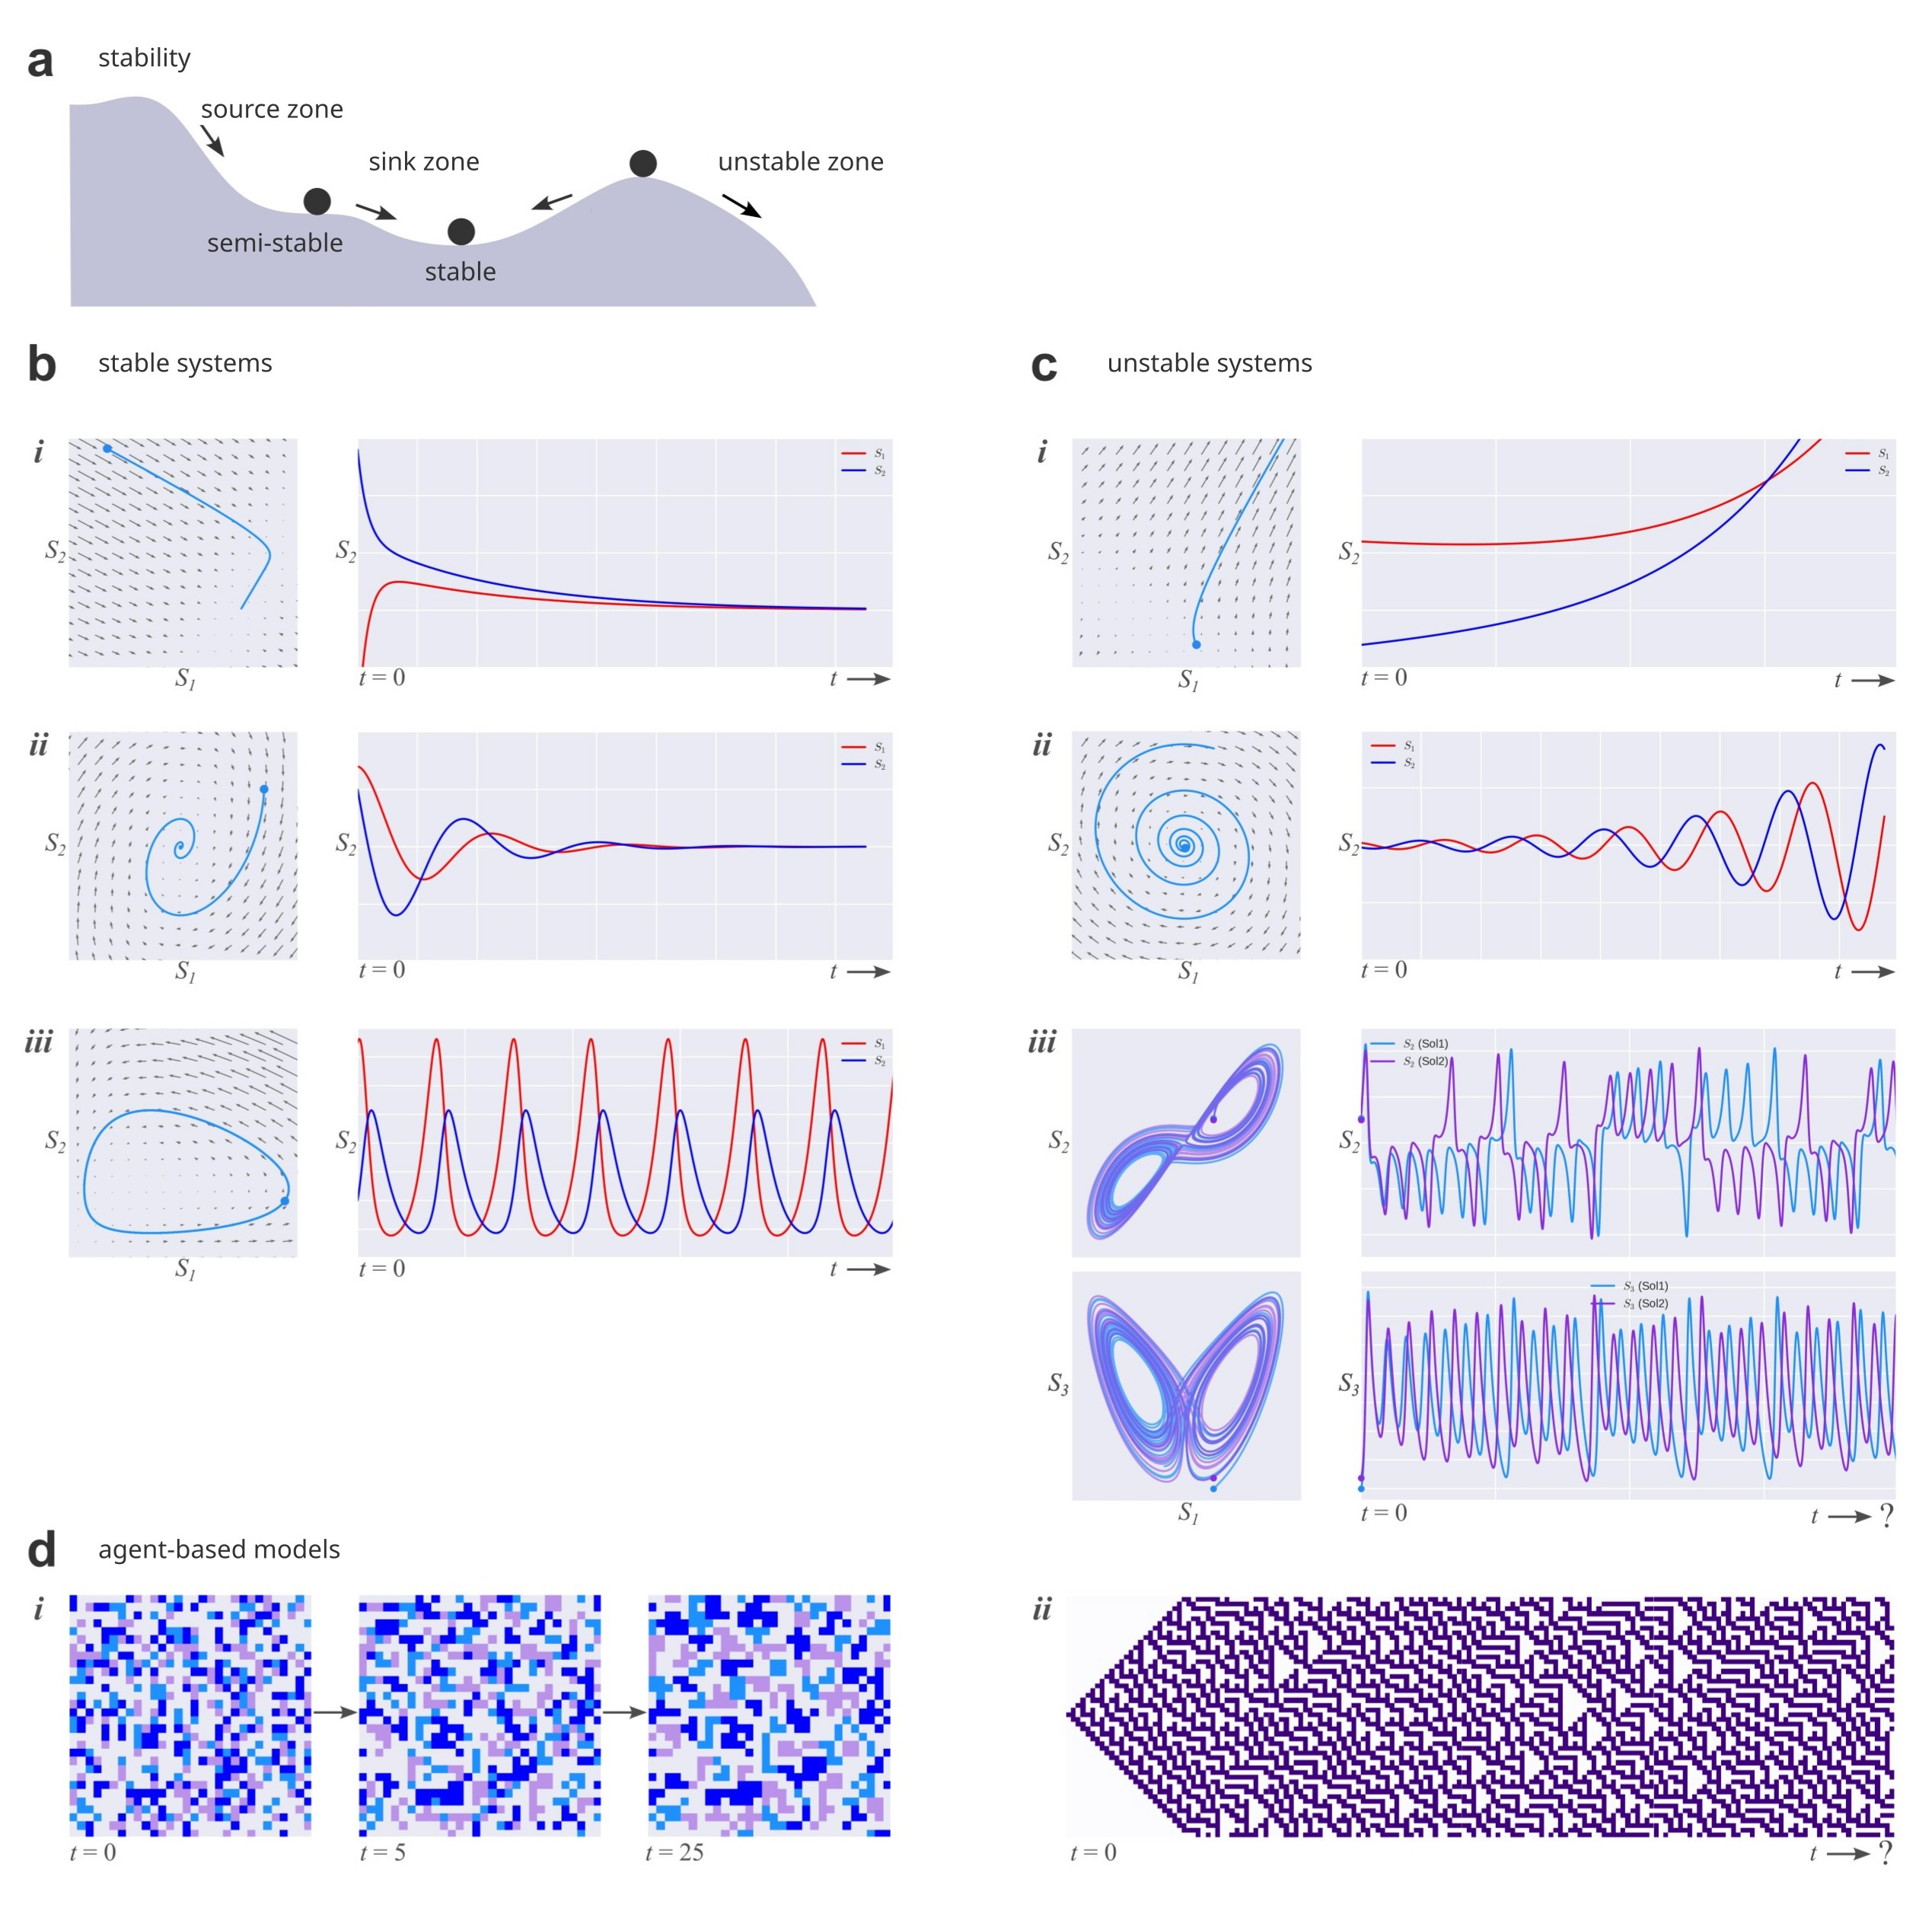
\includegraphics[width=0.95\linewidth]{figs/fig_systems_en.jpg}		
	\caption[Stability and behavior of systems.]
	{\textbf{---\;Stability and behavior of systems.} A \gls{system} is defined by a set of parts with relationships among them. Since it is the relationships that unify the whole, similar final behaviors emerge in different scientific fields.\;\textbf{a}\;---\;The behavior of a \gls{system} can be classified as stable or unstable, depending on its initial and boundary conditions. \;\textbf{b}\;---\;Stable systems with two elements ($S_1$ and $S_2$): exponential decay (detail \textrm{\textit{i}}) and damped oscillations (detail \textrm{\textit{ii}}) make an asymptotic movement toward an equilibrium point, being variations of the homogeneous linear \gls{system}. A stable \gls{system} can also exhibit eternal oscillations around the equilibrium point, as in the case of the Lotka-Volterra predator-prey \gls{model}, a non-linear \gls{system} (detail \textrm{\textit{iii}}). \;\textbf{c}\;---\;Unstable systems with two elements ($S_1$ and $S_2$): exponential growth (detail \textrm{\textit{i}}) and amplified oscillations (detail \textrm{\textit{ii}}) make a movement toward $+\infty$ or $-\infty$ (or both), also being variations of the homogeneous linear \gls{system}. Instability can also be chaotic, as in the Lorenz \gls{model}, a non-linear \gls{system} with three elements ($S_1$, $S_2$, and $S_3$; detail \textrm{\textit{iii}}). In the case of the chaotic \gls{system}, two solutions (in blue and purple) are visualized for very close initial conditions, but diverge in the long run (high sensitivity to initial conditions).\;\textbf{d}\;---\;Agent-based models illustrate that complex behaviors can emerge from simple interactions in the immediate neighborhoods of each agent. The Schelling \gls{model} (detail \textrm{\textit{i}}) illustrates the emergence of ordered clusters from random initial conditions. Wolfram's Rule 30 (detail \textrm{\textit{i}}) illustrates computational irreducibility: the only way to understand the final behavior of the \gls{system} is to simulate the \gls{model} step-by-step.
	}
\label{fig:sys:systems}  % use qualitative label			
\end{figure}

\par Although Bertalanffy admits that the General Systems Theory can be broadly applied from what he called \textit{verbal models}, he illustrates that \textit{formal models} of systems can be derived from a more or less general mathematical formulation. In this case, this formulation involves a \gls{system} of simultaneous differential equations. Thus, for $n$ elements characterized by a quantitative measure $S$:

\begin{linenomath*}
\begin{equation}
\label{eq:systems}
\begin{split}
    \frac{dS_1}{dt} &= f(S_1, S_2, ..., S_n)\\
    \frac{dS_2}{dt} &= f(S_1, S_2, ..., S_n)\\
    ...\\
    \frac{dS_n}{dt} &= f(S_1, S_2, ..., S_n)\\
\end{split}
\end{equation}
\end{linenomath*}
In other words, any variation in $S_i$ is a function of the overall state of the \gls{system}, which includes all other elements. This formulation also allows for the destruction of the relationship between the parts: it is enough to make the state $S$ of an element solely a function of itself, that is,  $dS_i/dt = f(S_i)$. In this case, the \gls{system} as an ontological entity ceases to exist, with the final state of the whole completely reduced to the overlay of the states of the individual elements. But when there are relationships, however trivial, Bertalanffy demonstrates that from the differential equations emerges a rich variety of \textit{final behaviors}, such as exponential growth or decay and processes described by the \gls{curve-log}, such as saturation and autocatalysis. With just two elements, the linear \gls{system} of constant coefficients takes the following general form:
\begin{linenomath*}
\[
\begin{split}
    dS_1/dt &= c_{11}S_1 + c_{12}S_2\\
    dS_2/dt &= c_{21}S_1 + c_{22}S_2\\
\end{split}
\]
\end{linenomath*}
In this simple \gls{system}, the Taylor series expansion allows solutions to be obtained for $S_1$ and $S_2$ through mathematical analysis. The different solutions demonstrate the emergence of different \textbf{stability conditions} (Figure \ref{fig:sys:systems}\,a). This can be visually represented graphically from a \textbf{phase plane} where the trajectories of the states of the two elements are drawn and also by the evolution of the variables in the time domain. Thus, the multiple configurations of values of the \gls{parameters} (coefficients) and also the initial conditions reveal the \textbf{\gls{atractors}} acting on the \gls{system}. For example, under certain conditions, the \gls{system} is stable and migrates from a \textit{source} to a final state ($S^*_1, S^*_2$), or node, in a \textit{drain}. This can occur smoothly or through \textbf{damped oscillations} (Figure \ref{fig:sys:systems}\,b, details \textrm{\textit{i}} and \textrm{\textit{ii}}). Under other conditions, the \gls{system} is unstable, eternally migrating, either in a fixed direction ($-\infty$ or $+\infty$) or through \textbf{amplified oscillations} (Figure \ref{fig:sys:systems}\,c, details \textrm{\textit{i}} and \textrm{\textit{ii}}). Alternatively, the \gls{system} may exhibit \textbf{stable oscillations}, remaining forever in a loop when viewed in the phase plane (Figure \ref{fig:sys:systems}\,b, detail \textrm{\textit{iii}}). A famous example of stable oscillations is the non-linear \gls{system} of Lotka-Volterra mentioned in Section \ref{sec:sys:represent}, which simulates the interaction between the populations of prey $S_1$ and the population of predators $S_2$:
\begin{linenomath*}
\[
\begin{split}
    dS_1/dt &= r_{1}S_1 - c_{1}S_1S_2\\
    dS_2/dt &= -r_{2}S_2 + c_{2}S_1S_2\\
\end{split}
\]
\end{linenomath*}
Where $r_1$ and $r_2$ are growth and decay rates, respectively. The \textbf{\gls{strange-atrc}} of this \gls{system} is illustrated in two phase planes in Figure \ref{fig:sys:systems}c, in detail \textrm{\textit{iii}}. The detail also illustrates two trajectories that started very close but take on different behaviors in the long run. On the other hand, the problem of computational irreducibility relates (mainly) to the application of \textbf{\gls{abm-models}}. The \gls{abm-models} represent systems through fundamental elements – the agents – that follow simple rules in their immediate neighborhood. When represented in a regular matrix, such as a board, these models are called \textbf{cellular automata}. An exemplary agent \gls{model} is the \textbf{\gls{model} of segregation by Schelling} \sethlcolor{pink}\hl{[todo:cite]}. In this \gls{model}, the agents have qualitative categories. At each time step, the agents evaluate their immediate neighborhood and decide whether to move or stay, depending on their tolerance rate with agents of different categories. This \gls{system} with simple rules spontaneously produces organized clusters, as illustrated in Figure \ref{fig:sys:systems}d, detail \textrm{\textit{i}}. In this line, Stephen Wolfram demonstrates that simple rules in certain systems can generate unpredictable complexity, accessible only through simulations that evaluate the \gls{system} \textit{step-by-step} \sethlcolor{pink}\hl{[todo:cite]}. This computational law arose from experiments with cellular automata that followed simple rules of Boolean conversion (from 0 to 1 and vice versa) based on binary representation. Some rules, such as \textbf{Rule 30}, exhibit computational irreducibility (Figure \ref{fig:sys:systems}d, detail \textrm{\textit{ii}}). Both \gls{chaos} and computational irreducibility convey the same message: these are issues that cast doubt on the \textit{predictive capacity} of theories when it comes to dynamic and non-linear systems. At the same time, they are concepts that reinforce the importance of empirical adequacy and estimation of epistemic uncertainties so that policies are based on \textit{evidence}, not just on \textit{theories}, as explored in the previous chapter.


\section{Dynamics} \label{sec:sys:dynamics}

\par The advent of the \gls{paradigma} sistêmico in the 1960s allowed for the emergence of the discipline of \textbf{\gls{sys-dyn}}, which is, in fact, a fusion of control engineering with management science and decision-making. \gls{sys-dyn}, as the name indicates, studies the evolution of complex systems over time. Furthermore, John Sterman argues that \gls{sys-dyn} is fundamentally a method for \textit{learning} about the behavior of complex systems \cite{sterman2000}. As emphasized in the second epigraph of this chapter, Sterman asserts that models ultimately allow for gaining \textit{insights} into the structure and behavior of systems, exploring \textbf{\gls{leverage-pts}} to achieve desired outcomes in policy formulation and decision-making. The ability of a \gls{model} to accurately predict the state of a given \gls{system}, from this perspective, is not as important as understanding its functioning and developing action strategies. The creation of this discipline is attributed to Jay Forrester (1918 - 2016), who sought to understand the behavior of systems from a technological and managerial perspective, that is, focused on solving problems and achieving pre-established goals, from capturing a market share by an industry to reducing the concentration of greenhouse gases in the atmosphere. This is illustrated by his account that the fundamental ideas of this discipline emerged from a challenging industrial problem at \textit{General Electrics}, related to long-term fluctuations in jobs. After studying the decision-making processes of the industry, he used a simple simulation, with pencil and paper, which revealed a potential for oscillations in the internal organization of the \gls{system}:

\begin{adjustwidth}{100pt}{0pt}
\medskip
\small (...) even with constant incoming orders, one would get employment instability as a consequence of commonly used decision-making policies within the supply chain. That first inventory-control system with pencil and paper simulation was the beginning of the System Dynamics field – Jay Forrester \cite{forrester2007}.
\medskip
\end{adjustwidth}

\par Despite its beginning with pencil and paper, \gls{sys-dyn} clearly requires the use of digital computers to simulate highly complex models in industrial, urban, social, economic, environmental, and global contexts. A global application example is the world model \texttt{World3}, whose simulations were explored by Donella Meadows in \textit{Limits to Growth}, who was part of Forrester's research group at MIT. Currently, the application of concepts and the construction of \gls{sys-dyn} models are typically carried out using software such as \texttt{Stella} and \texttt{Vensim}, which utilize advanced graphical interfaces to facilitate the development of complex systems.

\par \gls{sys-dyn} formalizes the basic architecture observed in hydrological and environmental models. This architecture, in philosophical terms, is a singular ontology that consists of \textbf{\gls{compart-models}}, illustrated in Figure \ref{fig:sys:dynamics}a. In \gls{hydrology}, it corresponds to the reservoir or "bucket" model. This approach has consolidated in the environmental field, primarily due to the ease of \gls{abstraction} and the (relative) low computational demand. Another contributing aspect is that empirical evidence about environmental processes often results from aggregated processes, such as the flow of a river or the concentration of a substance in water or air, a fact that is changing with the advent of high spatial and temporal resolution remote sensing technologies. However, Sterman argues that compartment models are not the only form of representation in \gls{sys-dyn}. It also allows for architectures with disaggregated, heterogeneous, or even individualized parts, such as the previously mentioned \gls{abm-models} \cite{sterman2018}. In light of this, Sterman establishes a pragmatic attitude, arguing that the decision regarding the architecture of the \gls{model} should be considered from the perspective of the problem being evaluated, but without losing the ability to manage the \gls{model} with ease. As an example, he mentions that the SIR epidemiological model\footnote{The acronym SIR stands for Susceptible, Infectious, and Recovered.} is a \gls{compart-models} that exhibits practically the same aggregated final behavior as any other more detailed version. The justification for introducing heterogeneities, such as age groups, spatialization, or even agents that follow more or less social distancing rules, should reside in the final purposes of the study, within the scope of relevant recommendations for policy formulation and decision-making. Otherwise, one incurs in a practically infinite regression of details: after all, why model only the host agents if it is possible to model their organs, cells, and even the bacteria or viruses themselves? Another relevant issue regarding detailed architecture is its high computational demand. Although currently accessible and somewhat seductive, Sterman emphasizes that highly detailed simulations with long simulation times introduce cognitive biases in the modeling process, especially in the iterative component. In this case, there arises resistance both to reviewing deeper conceptual aspects and to diagnosing the \gls{model} through sensitivity and uncertainty analyses, which require many simulations.

\par In the compartment architecture, the \textbf{\gls{causal-struct}} of the modeled \gls{system} is defined by the arrangement of compartments connected by flows that can be material (transfer rates) or informational (positive and negative \gls{feedback} loops). From the Aristotelian perspective, the \textit{matter} of the \gls{system} consists of the compartments, while the \textit{form} of the \gls{system} consists of the flows. Thus, two identical sets of compartments, when connected by different material and informational flows, reveal themselves to be completely different systems. In \gls{sys-dyn} jargon, the emphasis on form is often expressed by the fact that \textit{the \gls{causal-struct} of a \gls{system} defines its behavior}. The \gls{model} should initially be visualized through a \textbf{\gls{causal-diag}}, as shown in Figure \ref{fig:sys:dynamics}a. Here, it is crucial to properly establish the \textbf{\gls{bounds}} that the \gls{model} represents, that is, which flows beyond which the subsequent compartments do not have significant causal effects on the modeled \gls{system}\footnote{As it is a decision, the boundary design has the dangerous potential to be a premise of neglect, to use Musgrave's term.}. A compartment consists of a \textit{level} of a state variable $S$ that accumulates over time, meaning it has \textit{memory}. An easy way to identify a level is to consider what happens if the material flows cease: in this situation, the levels in the compartments continue to exist, inert. The only way to change the level is through the action of the material flows. The level in the compartments is governed by some \textbf{\gls{princip-conserv}}, generally the conservation of \textit{mass}\footnote{In environmental models, it is generally assumed that water is an incompressible fluid of constant density, which enables a simple volumetric balance of water.}. In practice, this implies the application of a \textbf{\gls{eq-balance}}, where any variation in the level of a compartment results from the net effect of the input rates (positive) minus the output rates (negative). Mathematically:
\begin{linenomath*}
\begin{equation}
\label{eq:balance}
\frac{dS}{dt} = I - O 
\end{equation}
\end{linenomath*}
\par In which the material input flows $I$ and output flows $O$ are rates of change of the level $S$, and have units of $S$ divided by the adopted time unit. A compartment can have multiple input and output flows, with Equation \eqref{eq:balance} being the simplest possible version. These flows are defined as \textit{functions} of both the \textbf{state variable} $S$ (when feedback exists) and of \textbf{\gls{exo-vars}} $\Upsilon$ (outside the system boundaries\footnote{In environmental models, the \gls{exo-vars} are generally referred to as \textbf{external forcings} of the \gls{system}. In a typical hydrological \gls{model}, for example, precipitation is an exogenous variable.}) and a set of \textbf{\gls{parameters}} $\Theta$ (constants adjusted to reproduce the expected behavior of the system). In general terms:
\begin{linenomath*}
\begin{equation}
\label{eq:flows}
\begin{split}
    I &= f(S, \Upsilon_{I}, \Theta_{I})\\
    O &= g(S, \Upsilon_{O}, \Theta_{O})\\
\end{split}
\end{equation}
\end{linenomath*}
By including \gls{feedback}, the equations that define the material flows also capture the flows of \textit{information} that connect the compartments. Ultimately, they capture the structure of the \gls{system}, and thus, its final behavior. The behavior of the \gls{system} is so sensitive to them that, to some extent, the flow equations become intertwined with much of the hypotheses postulated by the \gls{teoria} that the \gls{model} is conveying\footnote{Evidently, the underlying \gls{teoria} is also represented by the instantiated compartments, by the boundary design, and even by the balance equations.}

\par Equation \eqref{eq:balance} expresses the balance of a compartment as an instantaneous and \textit{continuous} process over time, which generally corresponds to the expectations for the modeled \gls{sys-target}. For example, the volume of water in a bathtub that is being filled by a faucet increases continuously, not in discrete jumps. Other systems, such as the population in an ecological \gls{model}, exhibit discrete transitions over time as new generations replace the previous ones. In one way or another, it is impossible to program a digital computer to solve continuous differential equations directly, necessitating the application of numerical methods. This technological limitation of digital computers, while allowing significant advances in other aspects, such as multifunctionality, leads to the so-called \textbf{\gls{problem-numerics}}. In essence, this problem consists of the \textbf{\gls{integration-error}} associated with the numerical scheme used in modeling. In the case of the balance, this problem involves the difficulty of accurately determining the level $S_{t+1}$ from the known level $S_t$ and the selection of a time interval $\Delta t$. After all, how do you calculate the average of the input and output flows during the time interval? Especially when there is \gls{feedback}, any minimal variation in $S$ directly influences the rates of input or output flow. In light of this issue, Jay Forrester advocates the need to sacrifice the numerical accuracy of simulated results in favor of gaining useful knowledge about the \gls{sys-target} \cite{forrester1964}. Forrester's guidance, which can be viewed as a \textit{pragmatic convention}, suggests defining a time interval $\Delta t$ that is sufficiently small relative to the time scale of the modeled flows and then applying the \textbf{\gls{method-euler}} for numerical integration. Figure \ref{fig:sys:dynamics}d illustrates the \gls{integration-error} in the numerical solution of the differential equation $dS/dt = -kS$ (a linear reservoir), whose analytical solution $S = S_0e^{kt}$ is easily obtained. In this case, the \gls{method-euler} was applied with different time intervals $\Delta t$, demonstrating the improvement in integration with smaller intervals. For more complex systems without an analytical solution, it is expected that adopting a sufficiently short time step will ensure that the flow between one moment and another is approximately constant.

\par The choice of the \gls{method-euler} for numerical integration is certainly controversial, as there are other numerical methods that are recognized as more efficient (such as the Runge-Kutta methods), but that require greater computational demand. John Sterman advances this debate by establishing the \textbf{\gls{princip-ins}}\footnote{The term principle of insensitivity is my own.}: a crucial test that a \gls{model} must pass is to demonstrate that different time intervals do not influence (for practical purposes) the results of the simulations \cite{sterman2000}. After all, the results of a \gls{model} sensitive to the time interval defined in numerical integration are devoid of theoretical meaning. As long as the \gls{model} shows numerical instabilities depending on the time step, it is necessary to adopt progressively smaller time steps until reaching behavior that is independent of the chosen time interval. In the extreme case that the behavior of a modeled \gls{system} fails to remain stable across the range of viable time intervals with the available technology, then one must consider using a more efficient numerical integration method. In the case of the \gls{method-euler}, the numerical arrangement of finite differences from Equation \eqref{eq:balance} exhibits the following form:
\begin{linenomath*}
\begin{equation} 
	\label{eq:balance_numeric}
	S_{t+1} = S_{t} + I_{t}\Delta t - O_{t}\Delta t \quad \forall t
\end{equation}
\end{linenomath*}
That is, it is assumed that the input flows $I$ and output flows $O$ are constant during the course of the time step $\Delta t$, with the value of the rates always computed at time $t$ and then \textit{extrapolated} to $t+1$. For a compartment with $N$ input flows and $M$ output flows:
\begin{linenomath*}
\begin{equation} 
	\label{eq:balance_numeric_expanded}
	S_{t+1} = S_{t} + \sum_{i}^{N} I_{t, i}\Delta t - \sum_{j}^{M}O_{t, j}\Delta t \quad \forall \; t
\end{equation}
\end{linenomath*}
\par Starting from the indexing of $t$, the algorithm to simulate the \gls{system} on a computer basically consists of inserting Equation \eqref{eq:balance_numeric} within a loop\footnote{Note that, depending on the simplicity of the \gls{system}, a typical spreadsheet can perform the computation, where each row of the table consists of a time step.}. This loop then iterates through all values of $t$, incrementally calculating the states of the levels and subsequently updating the value of the flows based on the values from the previous step. In addition to the flow balance equations, Forrester suggests that a \gls{proced-model} of a \gls{system} (i.e., the computer code itself) should also include \textbf{\gls{eq-aux}} and \textbf{\gls{eq-sup}}. The \gls{eq-aux} are derived directly from the balance and flow equations, implemented to simplify the understanding of the computational steps by humans. The \gls{eq-sup}, on the other hand, define variables of interest that are not part of the modeled \gls{system}, such as statistics accumulated over time or in moving time windows.

% figure
\begin{figure}[t!] % place figure in the page
	\centering				
	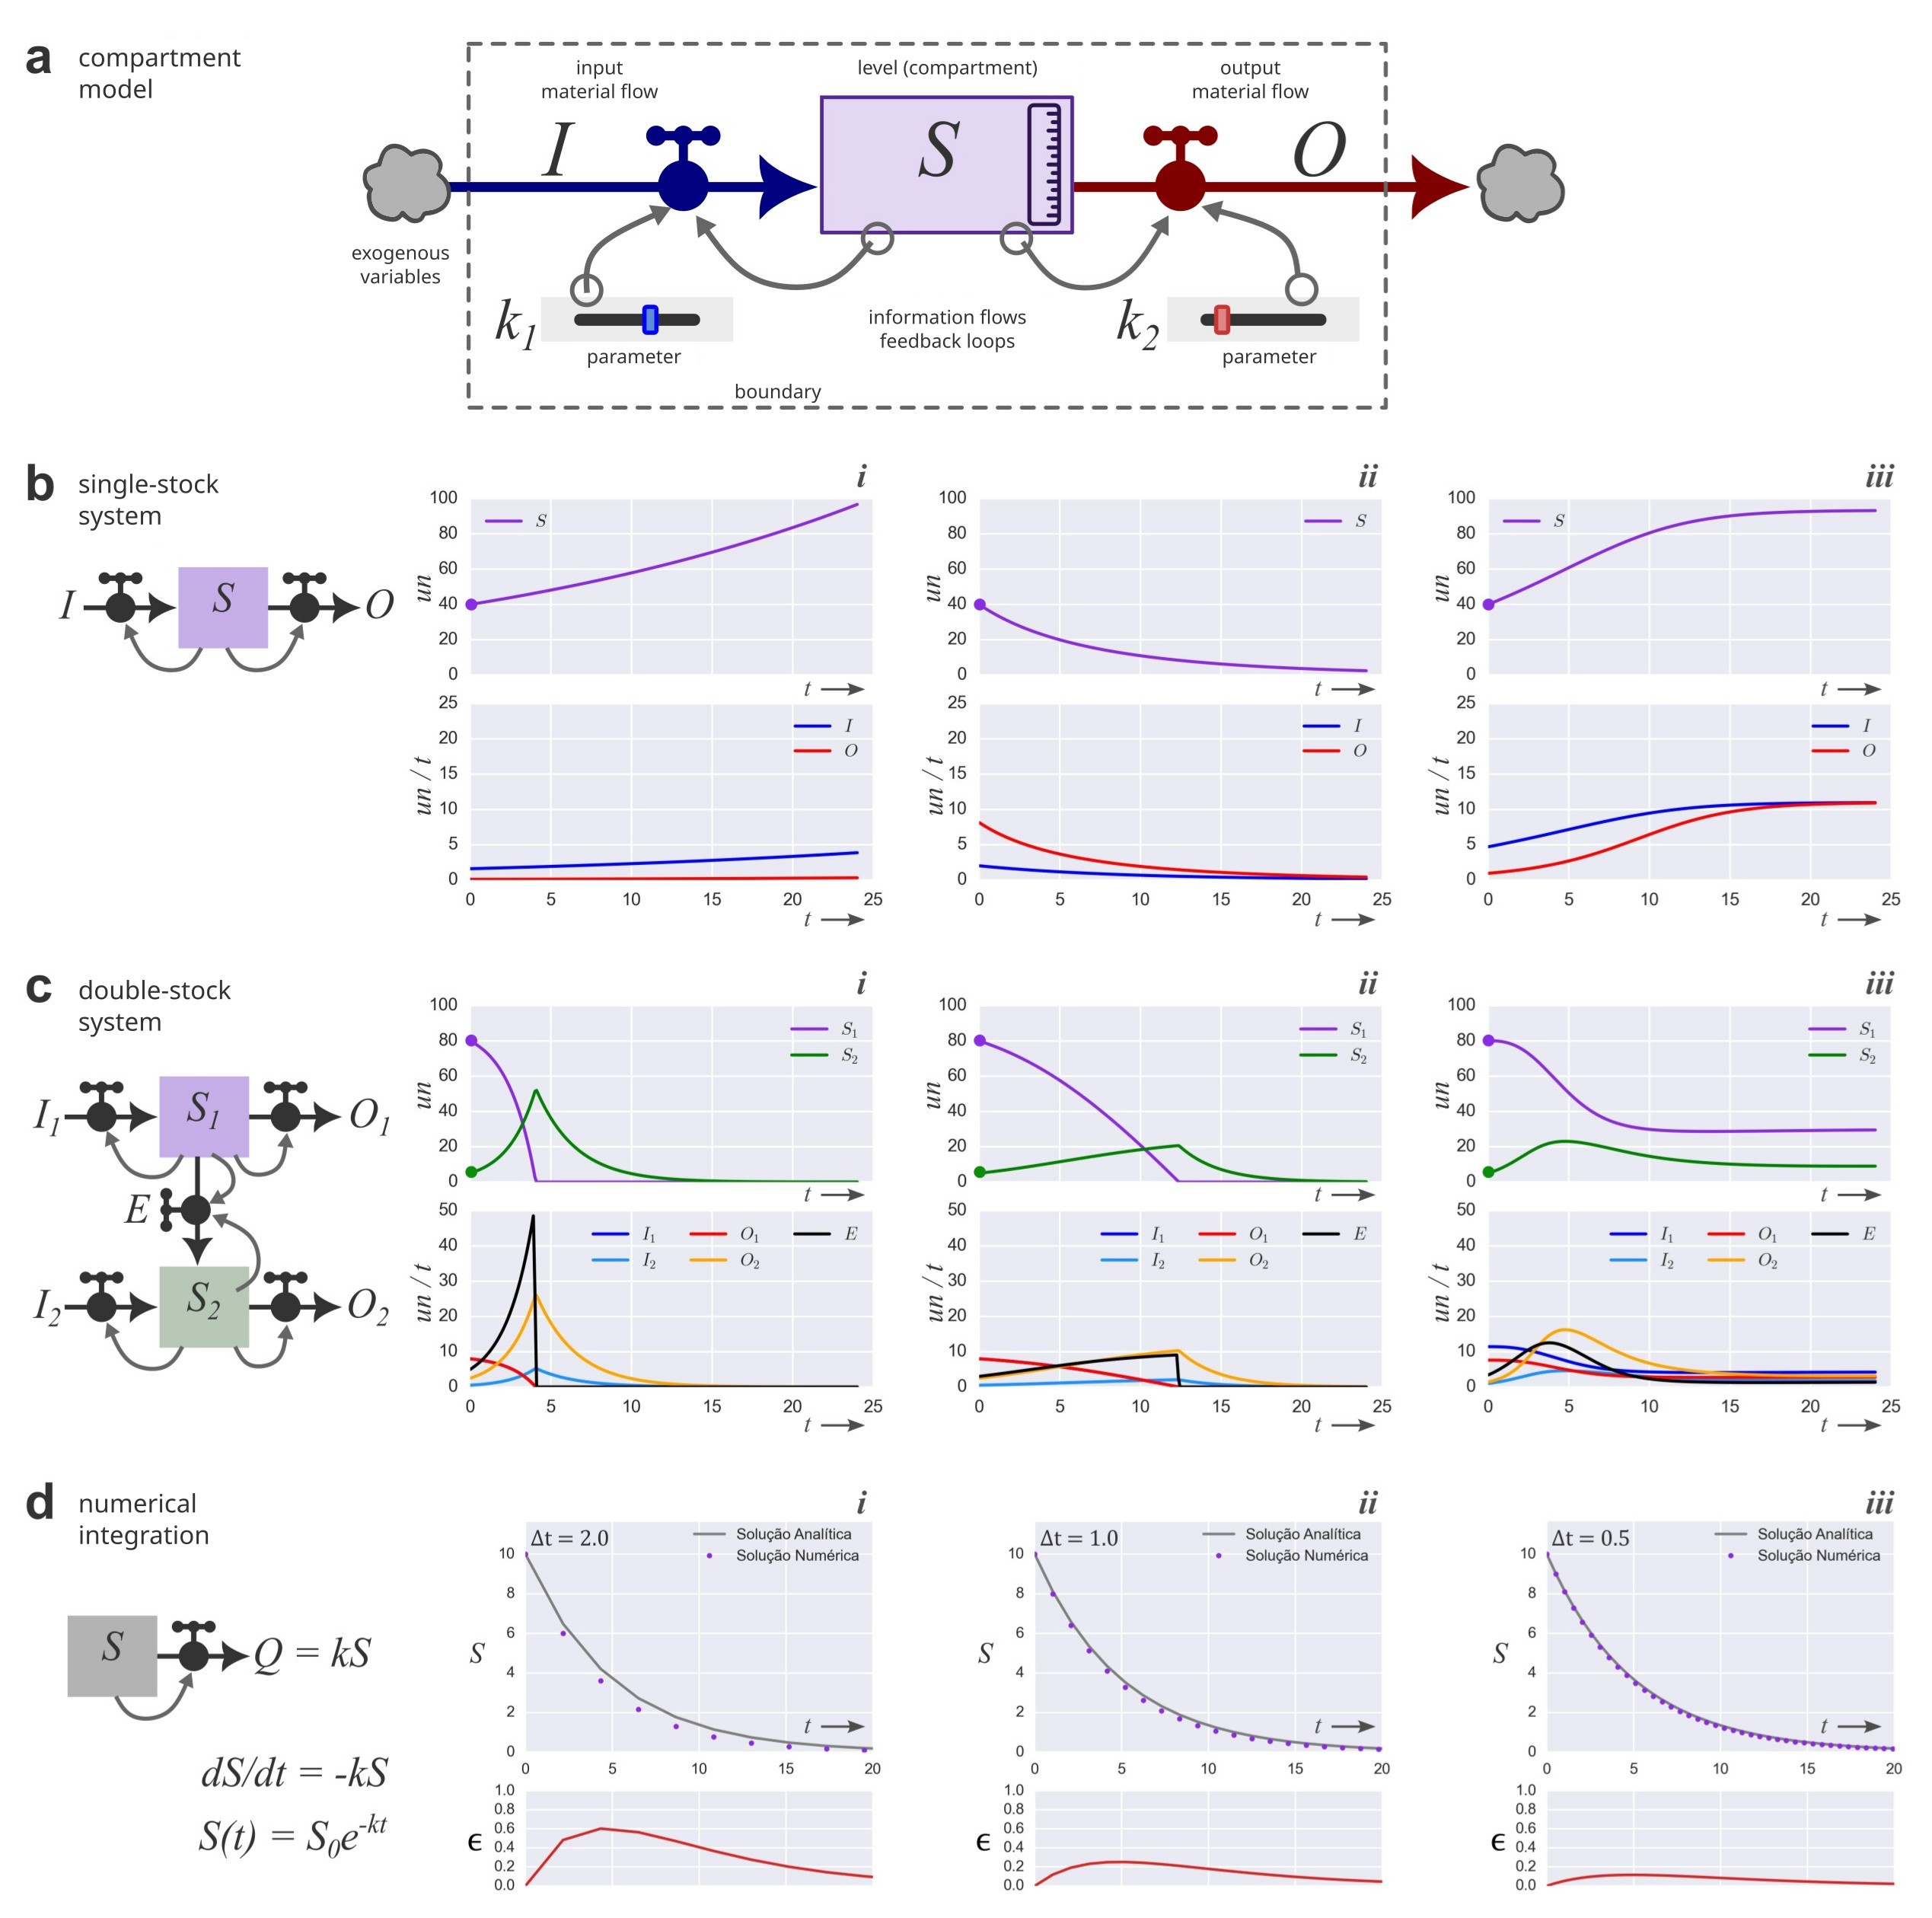
\includegraphics[width=0.95\linewidth]{figs/fig_dynamics_en.jpg}		
	\caption[\gls{sys-dyn} and the \gls{compart-models}]
	{\textbf{---\;\gls{sys-dyn} and the \gls{compart-models}.}\; The \gls{compart-models} consists of the basic architecture for constructing models within \gls{sys-dyn}. The \gls{system} is solved numerically, revealing complex patterns.\;\textbf{a}\;---\;Causal loop diagram: the level of the compartment $S$ changes due to the action of material inflows $I$ and outflows $O$. Information flows relate the level to the material flows through \gls{feedback}, which is regulated by \gls{parameters} of the \gls{model} (such as $k_1$ and $k_2$). The \textbf{boundary} of the \gls{system} should not neglect significant feedbacks with the \gls{exo-vars}.\;\textbf{b}\;---\;Simulations with the single stock \gls{model}, with different dominances between material inflows and outflows: exponential growth (detail \textrm{\textit{i}}); exponential decay (detail \textrm{\textit{ii}}), and; \gls{curve-log} (detail \textrm{\textit{iii}});\;\textbf{c}\;---\;Simulations with the double stock \gls{model}, where level $S_2$ depletes $S_1$ with an extraction flow $E$: overload and rapid collapse (detail \textrm{\textit{i}}); overload and delayed collapse (detail \textrm{\textit{ii}}), and; sustainable equilibrium (detail \textrm{\textit{iii}}).\;\textbf{d}\;---\;Numerical integration introduces the \gls{integration-error} $\epsilon$, which can be minimized with sufficiently short time steps $\Delta t$ (details \textrm{\textit{i}} to \textrm{\textit{iii}}). The overall behavior of the \gls{system} should not be sensitive to the time step $\Delta t$.
	}
\label{fig:sys:dynamics}  % use qualitative label			
\end{figure}

\par As previously mentioned, understanding the \textit{structure} of a modeled \gls{system} is key to predicting its \textit{behavior}. In this regard, the \gls{struc-iso} postulated by Bertalanffy becomes, within the realm of \gls{sys-dyn}, what Donella Meadows refers to as a \say{zoological garden of systems}: a set of systems that exhibit \textit{archetypical behaviors}, which can be generalized across a wide range of real examples \cite{meadows2008}. A good starting point in this context is to consider the simplest possible \gls{model}, which is one that has a single compartment, governed by Equation \eqref{eq:balance} (Figure \ref{fig:sys:dynamics}b). Although simple, different behaviors manifest depending on the \textit{dominance} of one flow over another. In the case where the inflow $I$ predominates over the outflow $O$, the level $S$ of the compartment will tend to increase (detail \textrm{\textit{i}} in Figure \ref{fig:sys:dynamics}b). If there is positive \gls{feedback}, the pattern will be that of \textbf{\gls{curve-exp-grw}}. Conversely, if the outflow predominates, the tendency will be for the level $S$ to decrease (detail \textrm{\textit{ii}} in Figure \ref{fig:sys:dynamics}b). Here, the existence of \gls{feedback} produces \textbf{\gls{curve-exp-dec}}. A concrete example of this archetypical \gls{system} is a culture of cells (such as bacteria or fungi), growing on a Petri dish without significant nutritional limitations. The more microorganisms reproduce (inflow), the more new generations are added to the total population, which grows exponentially. Simultaneously, the increasing confinement of cells leads to the accumulation of toxic waste from their own metabolism, which also increases mortality (outflow). These two flows act as a \textbf{\gls{loop-rei}} and a \textbf{\gls{loop-bal}}, competing for dominance over time, producing patterns more intricate than mere growth or decay, such as the \textbf{\gls{curve-log}} (detail \textrm{\textit{iii}} in Figure \ref{fig:sys:dynamics}b).

\par A second step in this direction is to consider the behaviors that emerge from the \textit{coupling} of two or more compartments. Meadows explores the basic \gls{model} with two compartments, particularly when the level $S_1$ of the first acts as a source of inputs $E$ for the level $S_2$ of the second (Figure \ref{fig:sys:dynamics}c). This is the case, for example, when the previously mentioned cell culture has limited nutritional resources. In fact, this arrangement is the archetype of any \gls{system} producer-consumer, which includes the global economy itself (natural resources and capital). A notable pattern that emerges from this \gls{system} is the \textbf{\gls{curve-oac}}, which occurs when the \gls{loop-bal} in the consumption of available resources does not exist or is very weak, causing the level of the second compartment to rise rapidly until it exhausts its own source, resulting in a similarly rapid decline (detail \textrm{\textit{i}} in Figure \ref{fig:sys:dynamics}c). The introduction of \textbf{double feedbacks} and \textbf{activation thresholds} to mitigate or even suspend the consumption of resources can either delay the collapse (detail \textrm{\textit{ii}} in Figure \ref{fig:sys:dynamics}c) or establish a \textbf{sustainable equilibrium} in the long term\footnote{In the case of the global economy, this optimistic scenario is referred to as \textit{prosperous decline} by Odum and Odum \cite{odum2008}} (detail \textrm{\textit{iii}} in Figure \ref{fig:sys:dynamics}c). Moreover, the introduction of \textbf{delays} in the flow of information can produce stable oscillations (naturally damped) or unstable oscillations (amplified and chaotic) in the levels. It is easy to see that the complexity and diversity of behaviors grow exponentially as new compartments and feedbacks are introduced into the models. The advantage of \gls{sys-dyn}, with its strictly computational nature, lies in its ability to simulate the \gls{system} step by step from the basic relationships between the compartments, eliminating the need to explicitly solve systems of non-linear differential equations. Thus, patterns of growth, decay, saturation, collapse, and oscillations simply emerge.

\section{A prototype} \label{sec:systems:model}

\par With what has been presented so far, we finally arrive at a suitable position to introduce a prototype of a \gls{model} hidrológico. In this line, the aim here is to establish the basic implications that \gls{sys-dyn} brings to hydrological modeling through an exploratory and minimalist \gls{model}. Theoretical and practical deepening, both on hydrological processes and on more detailed models, will be articulated in the next chapter. 

\par As highlighted in Section \ref{sec:sys:process}, every modeling process begins from a \textit{\gls{model} perceptual}. Thus, the minimalist \gls{model} arises here from some perceptions, especially the one that a watershed has at least two different ways of \textit{responding} to rainfall events: one faster and the other slower. The \textbf{\gls{hydro-response}} fast manifests in the rises of rivers that occur after rains. The \gls{hydro-response} slow, on the other hand, is evident during dry times, when rivers continue to flow even after many days or even months without rain. In this line, it is assumed that the fast response is more related to surface processes, while the slow response is associated with subsurface processes. The first relationship derives from the perception that highly impermeable watersheds or those with shallow soils produce large runoff (fast response). Conversely, the springs of streams and wet areas in the valley bottoms of more preserved watersheds reinforce the perception of the role of groundwater in sustaining base flow in rivers during dry times. An important perceptual detail that we can introduce here is that not all rain produces a fast response, as it is necessary to surpass a certain \textit{activation level}, such as \gls{interception} of water in the canopy or filling the depressions in the terrain that are not connected. Once this threshold is surpassed, the incremental \textit{saturation} of the surface produces an increasingly greater fast response, which will only cease when the surface is again dry. This occurs due to the \textit{level of fragmentation} of the surface -- that is, more water is needed to connect isolated pockets of water with the available outlets (in channels or macropores). Regardless of the forms of response, water also needs to travel through a network of channels to reach the outlet of the watershed. This reinforces another relevant perception, that the movement of water implies an attenuation of the response pulses due to energy dissipation effects. Finally, one last perception refers to the outflow of \acrfull{et}. In this case, it is expected that transpiration from plants through the canopy is the initial flow, followed then by evaporation of water from the surface.

\par Once a \gls{percept-model} is established, we can move on to a \gls{concept-model} from the perspective of \gls{sys-dyn}. The diagram of this \gls{model} is displayed in Figure \ref{fig:sys:proto}a. Thus, the first step in this process is to define the \gls{bounds} of the modeled system. In the case of typical hydrological models, the aim is to represent a watershed, which is an area of land traversed by the \gls{hydro_cicle}. The watershed, therefore, is an open \gls{system} to water flows that enter through atmospheric precipitation $P$ (rain, snow, and dew) and to outflows, which can occur through both runoff $Q$ and \acrlong{et}, denoted here as $E$. Thus, the flows $P$ and $E$ are maintained as \gls{exo-vars}, obtained from \textbf{\gls{input-data}} and acting outside the boundary of the \gls{sys-target}. It is assumed, therefore, that the internal state of the \gls{system} does not exert causal influence over the value of these variables\footnote{This assumption becomes increasingly fragile as the scale of the watershed evolves from a small area to larger regions or continents \sethlcolor{pink}\hl{[todo:cite]} to cite examples and references.}. It is clear that, as an outflow, \acrlong{et} depends on the water available in the \gls{system}, but its \textit{potential} flow is determined without causal links. Runoff $Q$, on the other hand, is a flow calculated by the \gls{model} itself through the application of its flow equations. Models with this characteristic are often called "rain-runoff" models, although this designation obscures the fact that many other flows are calculated to estimate the outflow.

\par The second step in building a \gls{concept-model} involves configuring the reservoirs\footnote{In the context of hydrological models, I will use the term \textit{reservoir} as a synonym for \textit{compartment}.} of the \gls{system} under study. For this, it is essential to mobilize the concept of \gls{hydro-response} provided by the \gls{percept-model}. To keep the \gls{model} in a minimalist condition, we define only two response reservoirs: one for the fast response, $S_1$, and another for the slow response, $S_2$. These reservoirs are vertically coupled, so that the water must pass through the fast response reservoir (upper) before reaching the slow response reservoir (lower). This scheme aims to represent the water balance in the soil, intuitively relating the fast response to surface processes and the slow response to subsurface processes. However, due to the simplification of the \gls{model}, this interpretation should be considered with caution: the representation in only two reservoirs is essentially a synthesis of several subprocesses that could be more specifically defined in a more detailed \gls{model}. In addition to the coupled reservoirs, a third reservoir, $S_3$, collects both the fast and slow flows, acting as a filter over the signal of both. The purpose of this reservoir is to model the effects of attenuation and storage during the propagation of runoff through the channel network before reaching the watershed outlet. Just as in the case of the water balance in the soil, this reservoir encompasses several subprocesses that, in a more complex \gls{model}, could be explored in detail. Considering that the area of the watershed is constant, it is convenient, though not mandatory, to express the levels of the reservoirs $S_i$ in \textit{mm} of water column and the flows in \textit{mm}/$\Delta t$. The reservoirs $S_1$ and $S_3$ (surface and channel network, respectively) have unlimited total capacity, while the reservoir $S_2$ (soil and subsurface) reaches its maximum capacity from a certain level, such that:
\begin{linenomath*}
\begin{equation}
\label{eq:max_capacity}
S_{2, t} \leq s_{2,\text{max}} \quad \forall ; i, t
\end{equation}
\end{linenomath*}
Where $s_{2, \text{max}}$ is the \textit{maximum storage capacity} of $S_2$, a parameter expressed in level units (\textit{mm}).

\par The third step, finally, is to define the flow equations that govern the water balance in each reservoir. In this sense, all three reservoirs operate as a \textbf{\gls{linear-reserv}}, which implies that they exhibit an outflow $Q_t$ directly proportional to the level $S_t$, that is:
\begin{linenomath*}
\begin{equation} 
	\label{eq:linear_reservoir}
	Q_{i, t} = \frac{1}{k_{i}} \cdot S_{i,t} \quad \forall \;  i, t 
\end{equation}
\end{linenomath*}
Where $k_i$ is a parameter with time units that is equivalent to the mean residence time of the reservoir $S_i$. This implies that the \textit{greater} the value of $k_i$, the more \textit{slow} its emptying is, as illustrated in Figure \ref{fig:sys:proto}b (details \textit{i} and \textit{ii}). A \gls{linear-reserv} is analogous to a water tank with vertical walls and a porous outlet, which allows a laminar flow directly proportional to the water column. In the case of the fast response reservoir $S_1$, the outflow $Q_1$ is the flow of vertical transfer of water to the reservoir $S_2$, interpretable as the \textit{infiltration} from the surface into the soil, with the necessary effectiveness caveats. In the case of reservoir $S_2$, the outflow $Q_2$ is the very slow response of the watershed, interpretable as the \textit{base flow} that the soil produces directly into the drainage network. Finally, the outflow $Q_3$ is the final \textit{outflow rate}, resulting from the attenuation of the runoff through the propagation process. The rapid outflow from reservoir $S_1$, denoted by $R$, has a specific formulation, corresponding to a \gls{hipotese} of how rapid processes, such as \gls{sf-runoff}, develop in the watershed. Just like in the outflow of a \gls{linear-reserv}, $R$ is directly proportional to the stored level, with the difference that the level must exceed a minimum value $s_a$ before it begins to overflow:
\begin{linenomath*}
\begin{equation} 
	\label{eq:fast_response}
 R_{t} = 
\begin{cases} 
    0 & \text{if } \quad S_{1,t} \leq s_a\\
    c \cdot (S_{1,t} - s_a) & \text{if } \quad S_{1,t} > s_a
\end{cases}
\end{equation}
\end{linenomath*}
Where $s_a$ is the \textbf{activation level} of the fast response, a parameter of the \gls{model} expressed in level units; and $c$ is a \textit{runoff coefficient}, with units of $t^{-1}$. However, unlike the \gls{linear-reserv}, the value of $c$ is not constant, but rather a function of the level $S_1$ itself. For the purposes of this chapter, we will simply establish that the fast response $R$ results from a \textit{saturation process} of the reservoir $S_1$, such that:
\begin{linenomath*}
\begin{equation} 
	\label{eq:fast_coeff}
	c = \frac{(S_{1,t} - s_a)}{(S_{1,t} - s_a) + s_c} \frac{1}{\Delta t} \quad \forall\;t
\end{equation}
\end{linenomath*}
\par Where $s_c$ is the \textbf{fragmentation level}, a parameter with the same units as the level $S_1$ that regulates the speed of the saturation process. The level $s_c$ represents 50\% connectivity, so that the greater the value of $s_c$, the more slowly the saturation of the reservoir occurs. As the reservoir level increases, the runoff coefficient $c$ asymptotically approaches 1\footnote{Equation \eqref{eq:fast_coeff} presents a typical form of saturation processes found in distinct fields, such as the \textbf{Michaelis-Menten Equation} in the kinetics of chemical reactions.}, as illustrated in Figure \ref{fig:sys:proto}b (details \textrm{\textit{iii}} and \textrm{\textit{iv}}). The term $1/ \Delta t$ was retained in the definition of $c$ to clarify its units, even though it is effectively eliminated in the \gls{eq-balance} (Equation \eqref{eq:balance_numeric}). By substituting Equation \eqref{eq:fast_coeff} into Equation \eqref{eq:fast_response}, we arrive at the flow equation for $R$ (in the case of $S_{1,t} > s_a$)\footnote{A cautious look reveals that Equation \eqref{eq:fast_response_2} has exactly the same structure as the empirical formula of the CN method proposed by the Soil Conservation Service to estimate effective runoff from rainfall events and types of land cover. This is an intriguing fact that deserves further study.}:
\begin{linenomath*}
\begin{equation} 
\label{eq:fast_response_2}
 R_{t} = \frac{(S_{1,t} - s_a)^2}{(S_{1,t} - s_a) + s_c} \quad \forall\;t
\end{equation}
\end{linenomath*}

\par In this minimalist \gls{model}, the external \acrlong{et} flow $E$ acts on the soil water balance, affecting reservoirs $S_1$ and $S_2$, such that $E = E_1 + E_2$. The drainage of water, in this case, occurs from the bottom up, meaning that the flow $E$ only starts to act on the upper reservoir $S_1$ when the lower reservoir $S_2$ is empty. That is, the outflow $E_2$ in $S_2$ corresponds to the transpiration of plants, which removes water from the soil, and the outflow $E_1$ in $S_1$ corresponds to surface evaporation. Thus, it is noted that the reservoirs $S_1$ and $S_2$ are \textit{simultaneously depleted} by more than one outflow. For $S_1$, the outflows are $E_1$, $R$, and $Q_1$. For $S_2$, the outflows are $E_2$ and $Q_2$. This is a good point to introduce two practical problems in compartment models within \gls{sys-dyn}, which are the \textbf{\gls{problem-congest-outputs}} and the \textbf{\gls{problem-simult-deplet}}. The first problem consists of the difficulty in determining a given outflow $O_{t,j}$ that \textit{is also an input} in a compartment with limited storage capacity. In the case of the minimalist hydrological model, this occurs in the flow $Q_1$ (infiltration), which goes from $S_1$ (surface) to $S_2$ (soil and subsoil). However, since the reservoir $S_2$ is limited by $s_{2, \text{max}}$ (Equation \eqref{eq:max_capacity}), there is a negative \gls{feedback} from $S_2$ on $Q_1$, which can be interpreted by the notion that the infiltration flow is \textit{congestible} by the moisture present in the soil. After all, if the soil pores are already filled with water, it doesn't matter how much water is available for infiltration stored on the surface. The \textbf{\gls{flux-actual}} $Q_{1,t}$, thus, is obtained by confronting the \textbf{\gls{flux-pot}} outflow $Q^*_{1,t}$ with the \textbf{\gls{flux-max}} possible input to the next reservoir, which in the case of $S_2$ is defined by the \textbf{\gls{storage-deficit}} $D_{2,t}$ divided by the time step $\Delta t$:
\begin{linenomath*}
\begin{equation} 
	\label{eq:congest_1}
 Q_{1,t} = 
\begin{cases} 
    Q^*_{1,t} & \text{if } \quad Q^*_{1,t} \leq D_{2,t} / \Delta t\\
    D_{2,t} / \Delta t & \text{if } \quad Q^*_{1,t} > D_{2,t} / \Delta t
\end{cases}
\end{equation}
\end{linenomath*}
Where $D_{2,t}$ is calculated by:
\begin{linenomath*}
\begin{equation} 
	\label{eq:congest_2}
 D_{2,t} = s_{2, \text{max}} - S_{2,t}
\end{equation}
\end{linenomath*}
\par This solution can be generalized for other congestible outflows\footnote{In this context, it is worth noting that John Sterman argues against using conditional structures like \texttt{IF... THEN... ELSE} in simulation code, suggesting that an alternative for Equation \eqref{eq:congest_1} of the form $Q_{1,t} = \texttt{MIN}(Q^*_{1,t}, D_{2, t} / \Delta t)$ is more robust and readable \cite{sterman2000}.}. When a compartment with limited capacity has \textit{multiple} simultaneous inflows, then the solution needs to adopt an analogous (but inverse) approach to the other problem mentioned, which is the \gls{problem-simult-deplet}. This problem, in turn, consists of the difficulty in \textit{preventing negative values} in a level subjected to multiple outflows that is numerically integrated using the \gls{method-euler}. In a mathematically continuous \gls{system}, the various outflow rates smoothly act on a given level $S_t$, so it tends asymptotically toward zero. However, the \gls{method-euler}, by considering that the rates are constant during a discrete time interval $\Delta t$, introduces the risk that $S_{t+1}$ may take on negative values. The solution to this problem is to compute the outflows in three steps. In the first step, the total \textit{potential} outflow $O^*_t$ is calculated by summing the individual potential outflows. More generically, for $M$ potential outflows $O^*_{t,j}$:
\begin{linenomath*}
\begin{equation} 
\label{eq:simult_1}
 O^*_t = \sum_{j}^{M}O^*_{t, j} \quad \forall\;t
\end{equation}
\end{linenomath*}
Next, the \textit{actual} total outflow $O_t$ is determined by confronting the \gls{flux-pot} with the \textit{maximum} possible outflow, which is the value of the level $S_t$ of the reservoir divided by the time step $\Delta t$:
\begin{linenomath*}
\begin{equation} 
	\label{eq:simult_2}
 O_{t} = 
\begin{cases} 
    O^*_t & \text{if } \quad O^*_t \leq S_t / \Delta t\\
    S_t / \Delta t & \text{if } \quad O^*_t > S_t / \Delta t
\end{cases}
\end{equation}
\end{linenomath*}
Finally, the third step consists of calculating the values of the \textit{individual} actual outflows. Since the \gls{method-euler} assumes constant flow rates, the actual outflows are directly proportional to the \textit{allocation} of the potential outflows:
\begin{linenomath*}
\begin{equation} 
	\label{eq:simult_3}
 O_{t, j} = \frac{O^*_{t, j}}{O^*_t} \cdot O_{t} \quad \forall\;t
\end{equation}
\end{linenomath*}

{\renewcommand{\arraystretch}{1.5}% for the vertical padding
\begin{table}[t!]
    \centering	
    \tiny
    \sffamily
    \rowcolors{2}{white}{rowgray}
    \begin{tabular}{ 
        >{\raggedright\arraybackslash}m{1cm}  
        >{\raggedright\arraybackslash}m{6cm}  
        >{\raggedright\arraybackslash}m{1cm}
        >{\raggedright\arraybackslash}m{1cm}
        >{\raggedright\arraybackslash}m{2cm}}
        \toprule
        \textbf{Componente} & \textbf{Nome} & \textbf{Dimensão} & \textbf{Unidade} & \textbf{Categoria} \\ 
        \midrule
        $S_1$ & quick response reservoir (surface) & L & mm & level \\ 
        $S_2$ & slow response reservoir (subsurface) & L & mm & level \\ 
        $S_3$ & drainage network reservoir & L & mm & level \\ 
        $P$ & precipitation & L/T & mm/h & flow (exogenous)\\
        $E$ & potential \acrlong{et} & L/T & mm/h & flow (exogenous)\\ 
        $R$ & quick runoff ($S_1 \rightarrow S_3$) & L/T & mm/h & flow\\ 
        $Q_1$ & infiltration ($S_1 \rightarrow S_2$) & L/T & mm/h & flow\\ 
        $Q_2$ & slow runoff ($S_2 \rightarrow S_3$) & L/T & mm/h & flow\\ 
        $Q_3$ & outflow from $S_3$ & L/T & mm/h & flow\\ 
        $E_1$ & evaporation & L/T & mm/h & flow\\ 
        $E_2$ & transpiration & L/T & mm/h & flow\\ 
        $k_1$ & residence time of $S_1$ (surface) & T & h & parameter \\ 
        $k_2$ & residence time of $S_2$ (subsurface) & T & h & parameter \\ 
        $k_3$ & residence time of $S_3$ (drainage network) & T & h & parameter \\ 
        $s_a$ & activation level of quick response & L & mm & parameter \\ 
        $s_c$ & fragmentation level of $S_1$ & L & mm & parameter \\ 
        $s_{2,\text{max}}$ & maximum capacity of $S_2$ & L & mm & parameter \\ 
        \bottomrule
    \end{tabular}
    \caption[Summary of the hydrological \gls{model} prototype]{
    Summary of the hydrological \gls{model} prototype developed, listing the components of levels, flows, and \gls{parameters}. Due to the high degree of aggregation of the \gls{model}, the names and meanings of the components should be interpreted with caution, as they are in fact effective processes that could be better detailed and disaggregated in more complex versions. 
    }
    \label{tbl:prototype}
\end{table} 
}

\par Such problems, inherent to the computational nature of \gls{sys-dyn}, indicate the next step in the modeling process: the development of a \textit{\gls{model} procedural}, that is, a computer program. In the form proposed above, the \gls{concept-model} is simple enough to be implemented in a \textit{spreadsheet}, where the columns represent different storage and flow variables and the rows represent the time steps of the simulation. To follow the \gls{method-euler}, the formulas in the reservoir balance cells should refer to the previous row, in the flow columns. Some auxiliary columns should be created to implement the intermediate steps of the potential flows and maximum flows. Additionally, certain static cells should be kept isolated, such as the values of the \gls{parameters} $\Theta = \{k_1, k_2, k_3, s_a, s_c, s_{2, \text{max}}\}$, the initial conditions values $\textbf{S}_{t=0} = \{S_{1, t=0}, S_{2, t=0}, S_{3, t=0}\}$, and the \gls{exo-vars} values $\Upsilon = \{P_t, E_t\}$. A more robust alternative, however, is to implement the \gls{proced-model} from code, such as \texttt{C}, \texttt{Fortran}, \texttt{Python}, etc. A simple code structure should be based on the functional programming \gls{paradigma}, with three interconnecting steps: 
\begin{enumerate}
    \item importing \gls{input-data};
    \item processing the \gls{model}, and;
    \item exporting the output data.
\end{enumerate}
Each step has its typical characteristics and technical limitations, from defining the format of the data files to using efficient structures offered by the chosen programming language. In this regard, a code presents two fundamental advantages: one cognitive and the other operational. The cognitive advantage is that a code completely makes explicit the equations and the computational algorithm itself\footnote{Highly efficient codes often imply a sacrifice in readability, which reinforces the importance of supplementary materials such as documentation and comments.}. Spreadsheets and other graphical interfaces, in contrast, tend to obscure the formulas and the algorithm structure, making the \gls{proced-model} somewhat inaccessible in cognitive terms. The operational advantage, on the other hand, is that a code allows the \textit{nesting} of the simulation process in a larger hierarchy of processes, such as running batches (multiple simulations in series or parallel) and coupling with other models (where the output of one is used as \gls{input-data} in another). As we will see later, this operational advantage is essential for the diagnosis and research of models.

% figure
\begin{figure}[t!] % place figure in the page
	\centering				
	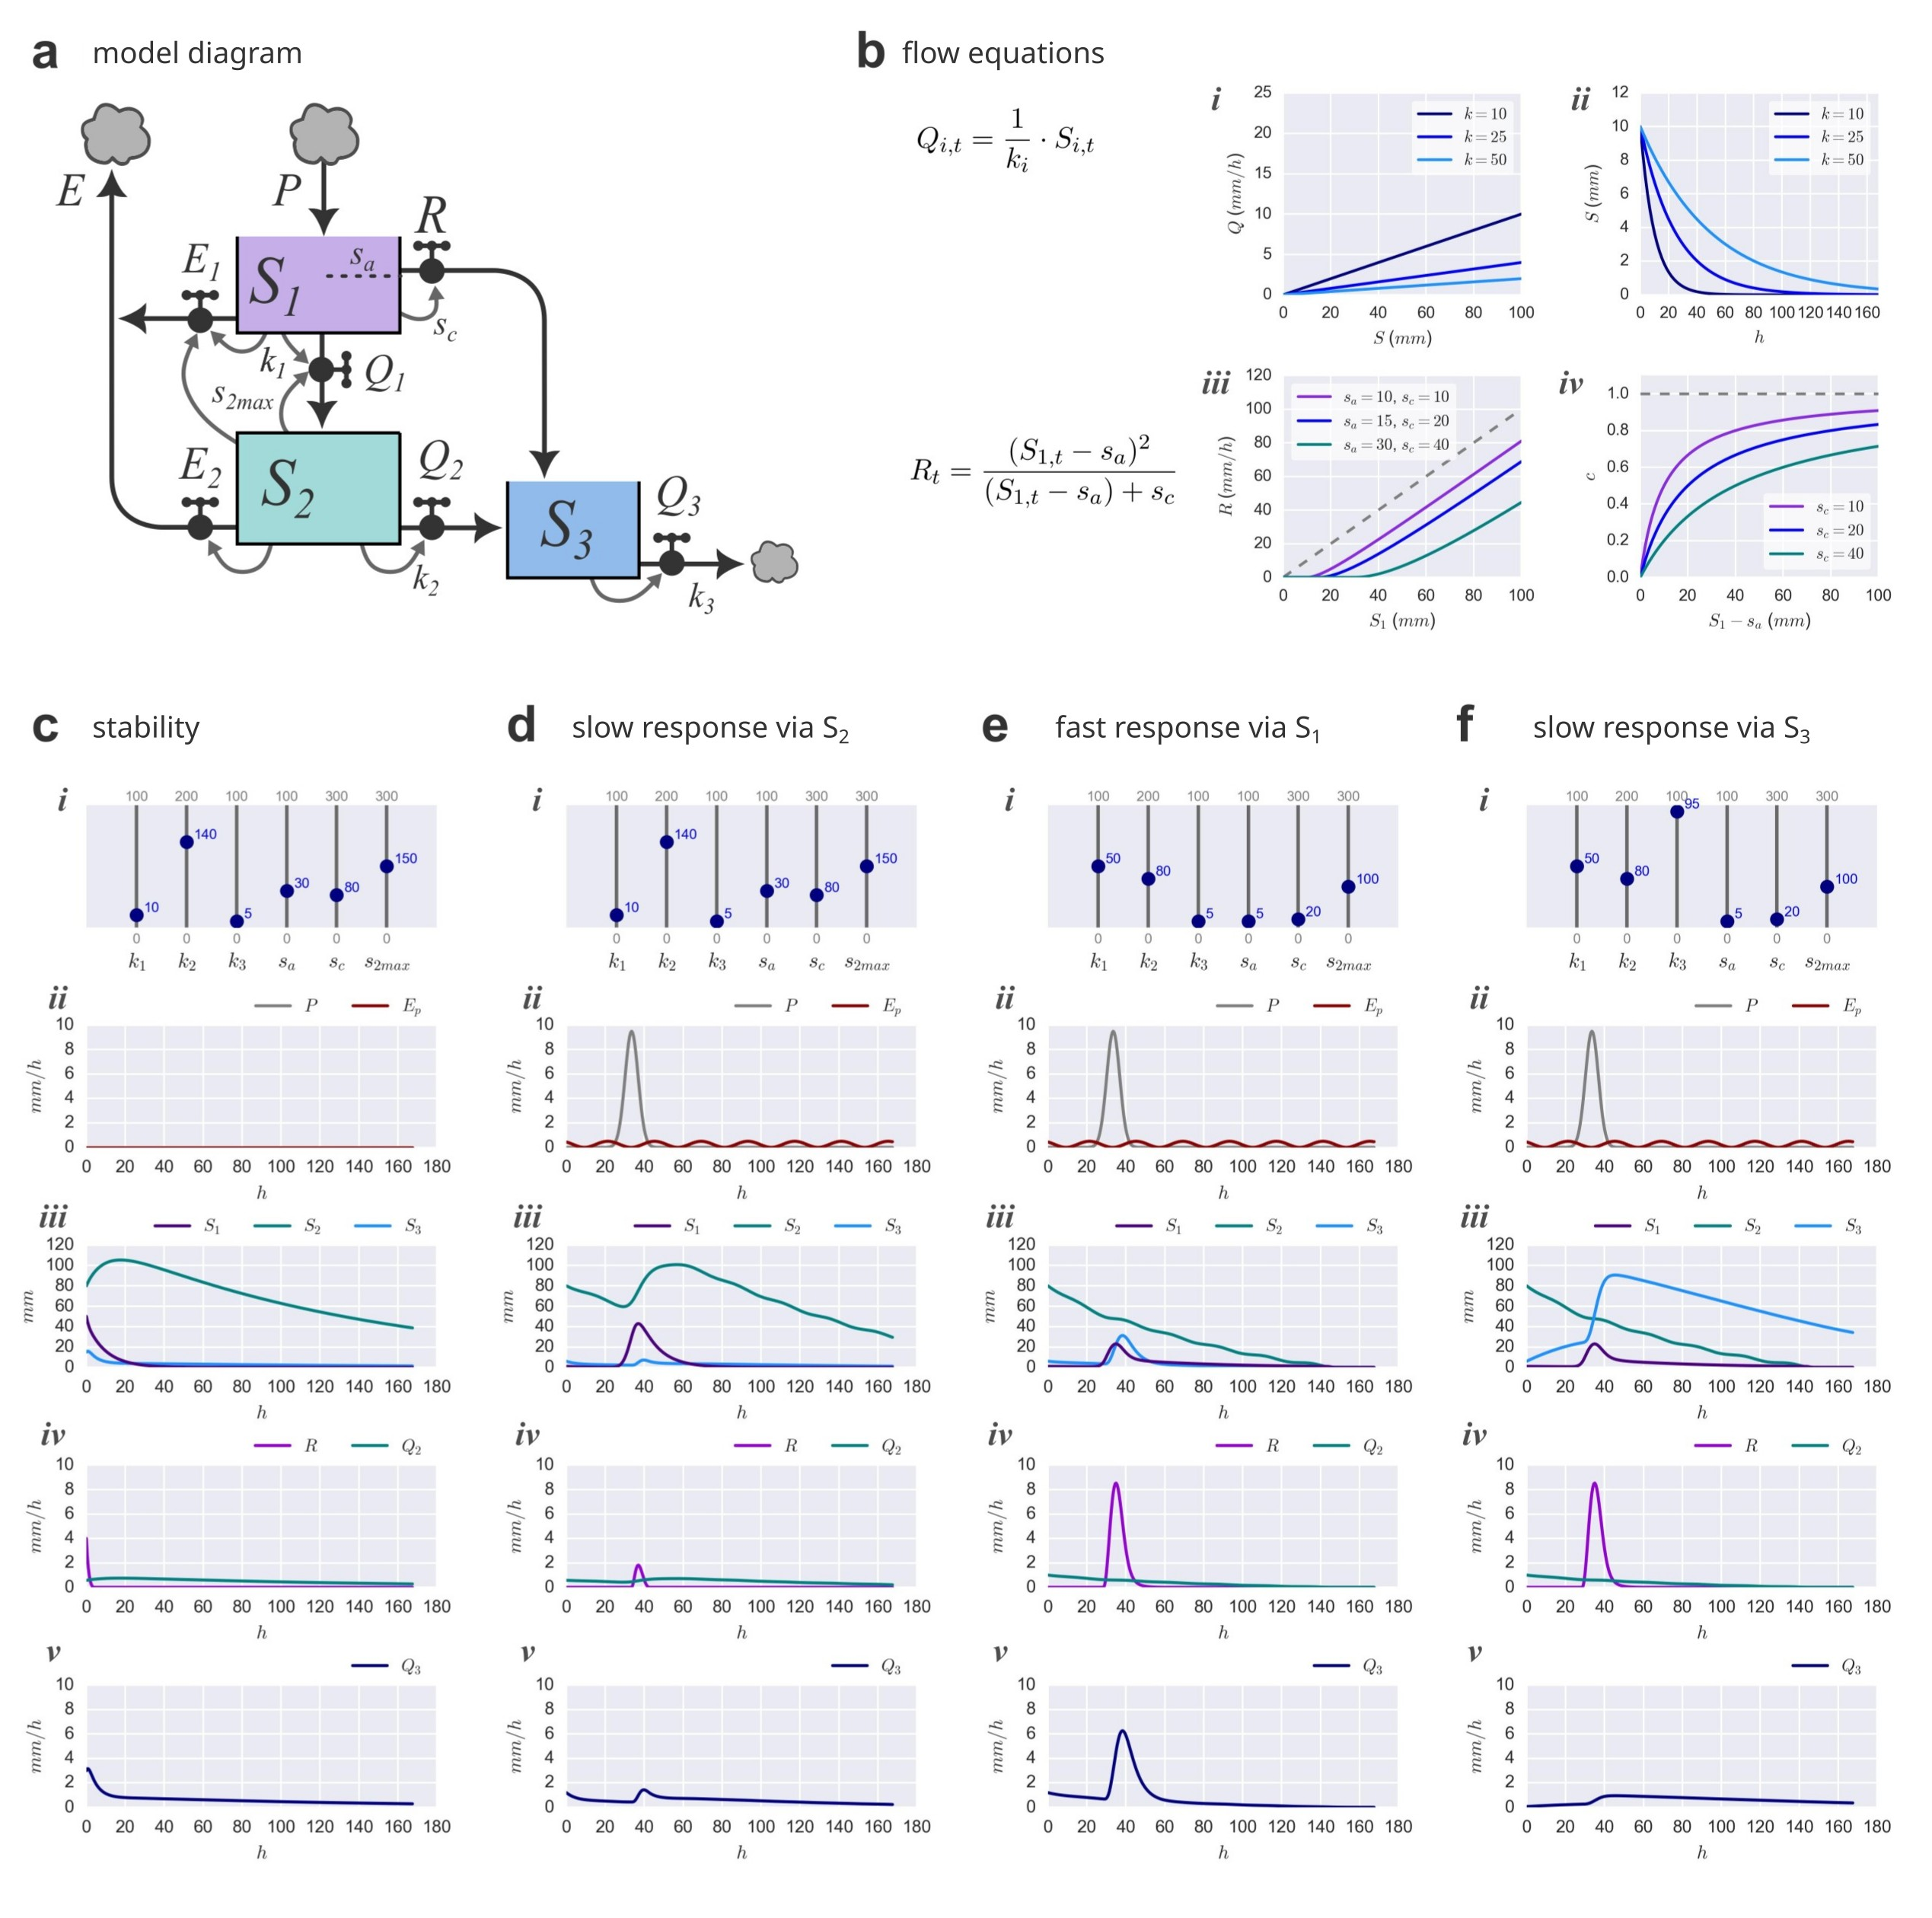
\includegraphics[width=0.95\linewidth]{figs/fig_minimodel_en.jpg}		
	\caption[A prototype of a hydrological \gls{model}]
	{\textbf{---\;A prototype of a hydrological \gls{model} and its behavior.}\;The \gls{model} is kept minimalistic for exploratory purposes.\;\textbf{a}\;---\;The structure of the \gls{model} is designed with three reservoirs ($S_1$, $S_1$, and $S_3$) to represent mechanisms of slow or fast \gls{hydro-response}. $S_1$ represents the surface, $S_2$ represents the subsurface, and $S_3$ represents the drainage network. With six \gls{parameters} regulating internal flows, the \gls{system} is subjected to the exogenous flows of evapotranspiration $E$ and precipitation $P$. The reservoir $S_2$ is the only one with limited capacity ($s_\text{2max}$).\;\textbf{b}\;---\;Two equations regulate the flows (Equation \eqref{eq:linear_reservoir} and Equation \eqref{eq:fast_response_2}). The exponential decay equation for the reservoirs ($Q_i = S_i/k_i$, detail \textrm{\textit{i}}), where $k_i$ is the residence time. The larger the value of $k$, the more slowly the reservoir empties (detail \textrm{\textit{ii}}). The quick response equation ($R = c\cdot (S_1 - s_a)$, detail \textrm{\textit{i}}) is similar, but $c$ results from a saturation process of the surface ($c = (S_1 - s_a)/(S_1 - s_a + s_c)$, detail \textrm{\textit{ii}}). This process is regulated by the activation threshold $s_a$ and the fragmentation level $s_c$.\;\textbf{c}\;---\;The \gls{system} shows stable behavior -- it empties by itself, even when $P$ and $E$ are null (detail \textrm{\textit{ii}}). In this case, $S_2$ showed a peak as water from $S_1$ infiltrated (detail \textrm{\textit{iii}}). But soon after, all reservoirs emptied.\;\textbf{d}\;---\;A configuration of \gls{parameters} (detail \textrm{\textit{i}}) that defines a slow response through the action of $S_2$ (subsurface). Here, a rainfall pulse $P$ with a maximum of 9.5 mm/h and a daily oscillation of $E$ (detail \textrm{\textit{ii}}) result in an attenuated flow $Q_3$ (detail \textrm{\textit{iv}}); $R$ has a maximum of only 2 mm/h, while the base flow $Q_2$ sustains the flow during most of the simulated period (detail \textrm{\textit{iii}}).\;\textbf{e}\;---\;A configuration of \gls{parameters} (detail \textrm{\textit{i}}) that defines a fast response through the action of $S_2$ (surface). The same pulse of $P$ and $E$ results in a typical hydrograph of $Q_3$, with a maximum of 6 mm/h (detail \textrm{\textit{iv}}); $R$ shows a maximum of 8 mm/h and the base flow $Q_2$ is extinguished in about 140 hours (detail \textrm{\textit{iii}}).\;\textbf{f}\;---\;A configuration of \gls{parameters} (detail \textrm{\textit{i}}) similar to (\textbf{e}), but defining a slow response through the action of $S_3$ (drainage network). The same pulse of $P$ and $E$ results in an attenuated flow $Q_3$ (detail \textrm{\textit{iv}}) -- the flow is sustained by damping in the drainage network.
	}
\label{fig:sys:proto}  % use qualitative label			
\end{figure}

\par Before conducting any computational simulation with the developed hydrological \gls{model} prototype, it is important to highlight some valuable aspects that the formalization of the \gls{percept-model} into a \gls{concept-model} brings. As mentioned earlier, \gls{sys-dyn} has an exploratory spirit that seeks not only to make reliable predictions about a \gls{sys-target} but also to use models to \textit{learn} about the behavior of this \gls{system}, thereby identifying useful \gls{leverage-pts} in decision-making. That said, let us consider for a moment that the \gls{teoria} conveyed by the proposed \gls{model} is \textit{justified}, which frees us from the issues raised in Chapter 1. If that is the case, what can we deduce \textit{a priori} about the behavior of the watershed? What are its critical \gls{leverage-pts} when considering, for example, the problem of water security\footnote{This problem will be explored in Chapter 4}?

\par In light of these issues, the first aspect to note is that \textbf{the \gls{system} is stable}, dominated by feedbacks that cause the levels of the reservoirs to \textit{tend towards zero}, as illustrated by the simulation in Figure \ref{fig:sys:proto}c. In other words: the reservoirs $S_1$, $S_2$, and $S_3$ empty on their own\footnote{In physical terms: through the action of gravity.}, even without any external action (when $P=0$ and $E=0$). Unlike ecological, social, and economic systems, no form of exponential growth or oscillations is expected from the proposed \gls{system}. A second aspect is to classify the final behavior of the \gls{system} in terms of sensitivity to the input flow $P$. At one extreme, we have low sensitivity behavior, characterized by the dominance of the slow response mechanism in $S_2$ and high residence time in $S_3$. The simulations in both Figure \ref{fig:sys:proto}d and Figure \ref{fig:sys:proto}f illustrate possibilities of this behavior. At the other extreme, we have high sensitivity behavior, characterized by the dominance of the rapid response mechanism in $S_1$ and low residence time in $S_3$, as shown in the simulation in Figure \ref{fig:sys:proto}e. Maintaining the proposed structure and the same exogenous flows $P$ and $E$, it is clear that behavior will strictly depend on the set of \gls{parameters} $\Theta = \{k_1, k_2, k_3, s_a, s_c, s_{2, \text{max}}\}$, although different values may eventually result in similar behaviors (high or low sensitivity). For example, it is possible to reduce the sensitivity of the \gls{system} by increasing both the activation threshold of the rapid response ($ \uparrow s_a$) and the residence time in the drainage network ($ \uparrow k_3$), or both simultaneously\footnote{This ambiguity is directly associated with the \gls{problem-equifinal}. As presented in Chapter 1, the largest number of possible empirical evidences should be employed to \textit{condition} the behavior of the \gls{model}.}. This leads us to the third and final aspect, which is the \gls{leverage-pts} of the \gls{system} in relation to practical problems, such as water security. For the purposes of this chapter, the problem of water security is defined as the difficulty in \textit{ensuring the availability of water in adequate quantity and quality} for human activities. Therefore, it is concluded that any leverage strategy in the \gls{system} should aim to reduce its sensitivity to the input flow, seeking a \textbf{\gls{regular-effect}}. In the soil water balance, this translates to reducing the dominance of the rapid response mechanism: increasing the activation threshold, reducing surface connectivity, and reducing surface residence time. In the case of the drainage network, the only available alternative is to increase residence time through detention basins, ponds, or even dams.

\par The aspects raised above illustrate that the simple deductive logic applied to the developed \gls{concept-model} allows for the identification of important \textit{insights} about the behavior and the \gls{leverage-pts} in the \gls{system}. Furthermore, if the \gls{model} captures the essence of the \gls{sys-target}, it is expected that more detailed versions do not eliminate the essence of the conclusions drawn, but rather introduce the necessary nuances in the decision-making process based on hydrological models, depending on the problem at hand. Heterogeneities in lithology, pedology, land cover, and topography should certainly expand the range of theoretical understandings and practical recommendations. Despite the leap observed between the \gls{percept-model} (\gls{mental-models}) and the \gls{concept-model}, it is clear that this reasoning can hide surprises from blind spots and non-intuitive interactions among the parts of the \gls{system}. Moreover, the assumption that the conveyed \gls{teoria} is justified was a provisional move: it is necessary to test the \gls{model} against empirical evidence. Thus, the only way to make stronger assertions is to simulate the \gls{model} using diagnostic techniques, which are presented next.

\section{Diagnosis} \label{sec:sys:diags}

\par The \textbf{\gls{model-diags}} consists of a vast set of techniques applied to evaluate the \textit{adequacy} of a \gls{model}. Before empirical justification, which is a crucial test, a \gls{model} needs to be adequate from the conceptual, technical, practical, and behavioral angles. After all, an extremely well-fitting \gls{model-stats} in empirical terms can be directly obtained with optimization techniques, such as machine learning. But what can one \textit{learn} about the \gls{sys-target} with a \gls{model-stats}? An overfitted \gls{model-stats} to the available data, for example, may be useful for \textit{interpolations}, but not for \textit{extrapolations}. Such a \gls{model} does not contribute much to understanding how the \gls{system} would \textit{behave} in response to a given leverage policy or a future scenario that has never been observed. The search for learning, in the context of \gls{sys-dyn}, implies that modeling is a process of \textit{deductive} inference, which requires a robust and reliable definition of the antecedent statements (main and auxiliary \gls{hipotese}) before producing their consequent statements (simulated results). In this regard, John Sterman suggests a list of twelve general strategies for diagnosing\footnote{Originally, he uses the term \say{model testing}, but here the term \say{test} will be reserved for when a \textit{rejection criterion} is explicitly defined.} these adequacies, displayed in Table \ref{tbl:tests}, enhancing Jay Forrester's initial proposals \cite{sterman2000}. However, given the highly practical nature of \gls{sys-dyn}, perhaps the diagnosis \textit{of zero order} of a model is to evaluate the \textbf{adequacy of the problem} it is being addressed. This primary diagnosis assesses whether the model was \textit{tailored} to answer the truly relevant questions of the practical problems at hand. Although obvious, this diagnosis can pose significant challenges, even forcing modeling teams to \textit{abandon} comfortable modeling strategies as the nature of the problem is understood more deeply. From the decision-making side, that is, the clients of model sellers, this type of diagnosis is essential to avoid uneconomical situations when the model sold is disproportionate. 

{\renewcommand{\arraystretch}{1.5}% for the vertical padding
\begin{table}[t!]
    \centering	
    \tiny
    \sffamily
    \rowcolors{2}{white}{rowgray}
    \begin{tabular}{ 
 >{\raggedright\arraybackslash}m{2.75cm}  
 >{\raggedright\arraybackslash}m{5cm}  
 >{\raggedright\arraybackslash}m{5cm}}
        \toprule
        \textbf{Diagnosis}$^*$& \textbf{Purpose}& \textbf{Procedures}\\ 
        \midrule

        \textbf{0. Problem Adequacy} & Diagnose if the model is suitable for the practical problem being addressed. & Explicitly state the questions implied by the problem that need to be answered by the model.\\
        
        \textbf{1. Boundary Adequacy} & Diagnose if the \gls{exo-vars} of the \gls{model} do not imply serious causal neglects. & Explicitly define the \gls{system} and its endogenous and exogenous variables in causal loop diagrams.\\         
        
        \textbf{2. Structural Adequacy} & Diagnose if the structure (including flow equations) aligns with the \gls{percept-model} and does not violate basic theoretical principles. The degree of aggregation also needs to be useful in practical terms.& 
        Inspect equations and causal diagrams; clarify decision-making questions related to expected outcomes.\\        
        
        \textbf{3. Dimensional Consistency} & Diagnose if the equations and \gls{parameters} are consistent and make sense concerning real phenomena.& 
        Inspect equations; dimensional analysis; rationalize the underlying \gls{teoria}.\\ 
        
        \textbf{4. Parameter Distribution} & Diagnose how distributions of values align with conceptual and empirical expectations.& Obtain prior distributions from expert opinion.\\        
        
        \textbf{5. Comparative Studies (System Families)} & Diagnose if the distribution of \gls{parameters} is consistent across target systems of the same family. E.g., different watersheds;& Obtain distributions of \gls{parameters} consistent with the largest possible number of system members (generalist \gls{model}).\\        
        
        \textbf{6. Integration Error} & Diagnose if the results are not sensitive to the time step and numerical integration method.& Reduce the time step; change the numerical integration method.\\        
        
        \textbf{7. Extreme Conditions} & Diagnose how robust the \gls{proced-model} is to very high or very low values.& Simulate the \gls{model} under synthetic conditions with extreme shocks to values.\\

        \textbf{8. Sensitivity Analysis} & Diagnose how variations in the \gls{parameters} of the \gls{model} affect the results, identifying critical \gls{parameters} for the behavior of the \gls{system}. & Apply exploratory techniques, such as the Monte Carlo Method, for random sampling in the \gls{parameters} space. Use search techniques to identify critical scenarios and reveal unusual leverage policies.\\
        
        \textbf{9. Anomalous Behavior} & Diagnose unexpected behaviors of the \gls{model} that may indicate formulation errors or important \textit{insights} about the modeled \gls{system}. & Subject the \gls{model} to encapsulation testing; discard.\\
        
        \textbf{10. Empirical Adequacy} & Diagnose if the \gls{model} can reproduce observed behaviors in the \gls{sys-target}, adjusting \gls{parameters} to improve adherence to empirical data. & Compare the outputs of the \gls{model} with observed data, using metrics like MAE, RMSE, and coefficients such as determination and KGE.\\
        
        \textbf{11. Surprising Behavior} & Diagnose if the modeling results surprise the target audience in some way, revising their \gls{mental-models}.& 
        Effectively communicate results; reveal nuances and details; demonstrate non-intuitive mechanisms.\\  
        
        \textbf{12. Positive Practical Impacts} & Diagnose if modeling has brought positive practical impacts on the decision-making process.& Prepare impact indicators from the \gls{model}; technical documentation; reproducibility.\\  
        \bottomrule
    \end{tabular}
    \caption[Model Diagnostics.]{
    \textbf{Model Diagnostics in the context of \gls{sys-dyn}.}\; --- \;Summary of the twelve \say{Model Tests} proposed by John Sterman, following the tests suggested by Jay Forrester. Adapted from Sterman \cite{sterman2000}.
    }
    \label{tbl:tests}
\end{table}
}

\par Among the conceptual diagnostics, it is essential to evaluate the \textbf{boundary adequacy}. As illustrated in the prototype of the hydrological \gls{model}, an important assumption is that the storage and flows of water in the watershed (the endogenous variables) do not influence precipitation and potential evapotranspiration (the exogenous variables). This assumption may be questionable for large watersheds, where evapotranspiration in one region converts into precipitation, either locally (cloud condensation nuclei \sethlcolor{pink}\hl{[todo:cite]}) or in other areas (flying river effect \sethlcolor{pink}\hl{[todo:cite]}). Thus, as one shifts from a \gls{loc-scale} to a continental scale, neglecting the causal interactions of the meteorological and climatic \gls{system} with terrestrial hydrological processes tends to become increasingly inadequate. Another basic conceptual evaluation is the \textbf{structural adequacy} of the \gls{model}, both in theoretical terms (physical principles) and practical terms (decision-making). The structure of the \gls{model} must ensure that physical principles, such as mass conservation, non-negativity of levels, and certain irreversible processes, are not violated. For example, Sterman describes an economic \gls{model} that produced remarkable results in simulating the leather market, but this occurred because the \gls{model} reverted produced leather \textit{back} into cows whenever necessary \cite{sterman2000}. Similarly, it is important to evaluate whether the level of aggregation of the \gls{model} meets the pre-established needs of the decision-making process. In hydrological modeling, the aforementioned prototype would hardly be useful for identifying priority action areas within a watershed, due to its highly aggregated nature.
 
\par Two other related conceptual diagnostics involve \textbf{dimensional consistency} and \textbf{parameter distribution}. This evaluation relates to the \textit{meaning} of the \gls{parameters} in the flow equations and the distribution of their values. When starting from a deductive logic, the flow equations need to make theoretical sense (after all, \textit{they convey a theory}), and their \gls{parameters} should have consistent names and units that are equivalent (at least in effective terms) to real processes. According to Sterman, \gls{parameters} and variables with names and units that do not make sense in the real world are \textit{symptoms that the \gls{teoria} about the \gls{sys-target} is poorly formulated}. Moreover, the values of the \gls{parameters} themselves also need to meet conceptual expectations. Since different combinations of \gls{parameters} can result in similar final behaviors (the equifinality problem), certain combinations of \gls{parameters} may be empirically adequate but theoretically questionable. For example, in a mountainous watershed without artificial reservoirs, one would expect low attenuation of the flow pulse in the drainage network, or at least lower than in flatter watersheds with floodplains. Thus, \textbf{comparative studies} between different systems but of the same \textit{family}, and the definition of prior distributions through \textbf{expert opinion}, help to discard inconsistent \gls{parameters} values\footnote{It is expected that expert opinion will \textit{inform} about the prior distribution of \gls{parameters} with qualitative empirical evidence from their perceptual models that have not been transformed into quantitative data. Still, care must be taken not to turn this process into a \textbf{confirmation bias}, keeping an openness for empirical anomalies to act as a means to refute the theories posited by the models. One way to achieve this is to maintain posterior probabilities within a minimum threshold.}.

\par On the technical side, a crucial diagnostic is the \textbf{test of numerical integration}, which was described in Section \ref{sec:sys:dynamics}. It is important to emphasize that \textit{no simulation is informative if its result stems from numerical instabilities}. Thus, this test consists of evaluating whether the behavior of the \gls{system} adheres to the \gls{princip-ins}. Another diagnostic in this vein is to subject the \gls{model} to \textbf{extreme and boundary conditions}, such as very high values of input and output flows. This is an assessment of technical robustness, as it is under these unusual (but possible) conditions that problems in the \gls{proced-model} may arise, such as errors in the numerical representation of data structures (\textit{overflow} and \textit{underflow}) and violations of non-negativity in the simulated levels. For example, a discrete level variable (like a population) can be instantiated by a data structure with positive, integer numbers of 16 bits—which offers interesting memory gains, unlike 64-bit floating-point numbers. However, this data structure has an upper numerical limit of 65535—values above this will wrap around to low numbers, causing an \textit{overflow} error that can render simulation results meaningless. In this case, it is necessary to ensure that a more efficient code does not compromise the robustness of simulations under extreme but feasible conditions.

\par Diagnostics that evaluate the behavior of the \gls{model} include \textbf{\gls{sal}}, \textbf{anomaly detection}, and \textbf{empirical adequacy}. These evaluations form a spectrum in terms of justification. On one side, \gls{sal} seeks to understand how the \gls{system} responds to changes in its elements, such as input flows and \gls{parameters} values. In this case, the approach is exploratory, without major commitments to justification. On the other side, empirical adequacy seeks to find the sets of \gls{parameters} that condition the modeled \gls{system} to reproduce the observed behavior. Clearly, this is the only test capable of pointing out the need for significant revisions in the modeling process, as it is here that the \gls{teoria} is directly confronted with the available evidence. Still, the rejection of the proposed \gls{model} is only possible through the modeling paradigm discussed in Section \ref{sec:epis:under} (Chapter 1), which applies an encapsulation test of a set of empirically adequate models. A purely confirmatory approach, in contrast, seeks to \say{calibrate} the \gls{parameters} of the \gls{model} in order to identify a single set of \gls{parameters} deemed adequate.

\par One way or another, behavior diagnostics generally require a broad assessment of the \textbf{\gls{space-params}} $\Omega_{\Theta}$, the mathematical space with $N$ dimensions created by the $N$ instantiated \gls{parameters} in the \gls{concept-model}. Here, a technical barrier arises, which is the \textbf{\gls{problem-dimens}}: the difficulty of thoroughly evaluating the \gls{space-params} $\Omega_{\Theta}$ in a reasonable simulation time. For example, consider a \textbf{\gls{brute-force}}\footnote{Also known as enumeration method or brute-force method.} approach with $M$ regular intervals across the estimated range for each parameter $\Theta_i$, with $i \in \{1, ..., N\}$. It follows that the number of simulations $n_s$ in a \gls{brute-force} approach is $n_s = M^N$. This number can grow exorbitantly quickly: with $M=100$, one would need to simulate the proposed hydrological \gls{model} ($N=6$) one trillion times, $100^6 = 1,000,000,000,000$. With a simulation time of one second, this evaluation would take around \textit{31 thousand years} to complete. A simulation time of one millisecond would require 31 years. To be practical, exploration in the \gls{space-params} $\Omega_{\Theta}$ should last a maximum of a few days, preferably a few hours or minutes.

\par More powerful computers greatly help in overcoming the \gls{problem-dimens}, but in practice, the sampling strategy also employs more efficient methods than \gls{brute-force}, which can be divided into \textbf{exploratory techniques} and \textbf{search techniques}, although they are largely related. Exploratory techniques are variations of the Monte Carlo Method, mentioned in Section \ref{sec:epis:bayes}, that perform random sampling over the expected value ranges for the \gls{parameters} $\Theta$. The goal here is merely to reveal regions of the \gls{space-params}. If a prior distribution for the \gls{parameters} is available (from expert opinion, for example), this sampling can be \textit{weighted by the density} of the distribution, which directs the exploration more towards certain regions than others. An efficient variation of the Monte Carlo Method consists of random sampling \textit{without replacement}, known as \textbf{\gls{lhs}}, which ensures a more spaced distribution of the sampled parameter sets, avoiding the risk of redundant samples. Search techniques, in turn, consist of optimization techniques aimed at identifying regions of the \gls{space-params} that meet predefined specifications regarding the behavior of the \gls{system}. In the jargon of Operations Research, these techniques maximize or minimize a given \textbf{\gls{obj-func}}. A wide variety of optimization algorithms can be implemented for this purpose, such as linear programming, dynamic programming, gradient ascent, evolutionary algorithms, Markov chains, etc. The criterion for selection, however, depends on various technical issues, especially in nonlinear models that exhibit objective functions with multiple local optima.

\par In \gls{sal}, exploratory techniques are applied to quantify the numerical sensitivity of each parameter. This analysis can be either \textit{local}, performed by varying one parameter while keeping the others constant, or \textit{global}, conducted through a more comprehensive exploration of the \gls{space-params} $\Omega_{\Theta}$ \cite{Saltelli2006}. Andrea Saltelli and colleagues emphasize the importance of the latter, demonstrating that only global analysis has the potential to capture interactions and synergies that emerge when a given set of \gls{parameters} changes simultaneously \cite{Saltelli2019}. However, \gls{sal} also employs search techniques in explorations designed to \textbf{discover critical scenarios} and reveal unusual leverage policies. To illustrate this approach, John Miller applied two optimization techniques (genetic algorithms and gradient ascent) to the \gls{model} \texttt{World3} used by Donella Meadows and colleagues in \textit{Limits to Growth}, in order to discover alternative scenarios for world population up to 2100 \cite{miller1998}. The results obtained from these searches indicated that it is possible to maximize the world population by up to six times the amount projected by Meadows' base scenario (4 billion, peaking at 9 billion in 2050), but it is also possible to minimize the population to half of the forecasted amount. These different modes of behavior of the same \gls{system} help to better understand the critical \gls{parameters} and flows necessary for policy development. For instance, a global population of 2 billion by 2100 might be desirable, not due to wars, pollution, and famine, but because of economic, technological, and cultural changes that improve people's quality of life.
 
\par On the side of empirical adequacy and anomaly detection, exploratory techniques are related to the uncertainty analysis of the \gls{parameters}. A method of particular relevance proposed in hydrological modeling is the \acrfull{glue} method, introduced by Keith Beven and Andrew Binley, which applies Bayes' Theorem (Equation \eqref{eq:bayes-model-multi}) with an informal likelihood function $\mathcal{L}(E|H)$ \cite{beven1992}. Thus, the posterior distribution of the \gls{parameters} is obtained by conditioning the prior distribution with the normalized histogram of the likelihood $\mathcal{L}(E|H)$. This histogram, in turn, is calculated from a robust exploration of the \gls{space-params} $\Omega_{\Theta}$. Search techniques, on the other hand, act to "calibrate" the \gls{model} by maximizing the likelihood $\mathcal{L}(E|H)$, resulting in a single set of \gls{parameters} deemed empirically adequate\footnote{In multi-objective approaches, the set of \gls{parameters} considered empirically adequate corresponds to a Pareto frontier.}. In any case, when it comes to models in \gls{sys-dyn}, the informal likelihood $\mathcal{L}(E|H)$ is usually equated to some point-to-point statistic or fit metric that seeks to measure the adherence of the simulated variables to the observed data. Therefore, the closer a simulated point $y_{M, i}$ is to its corresponding observed point $y_{O, i}$, the greater its empirical adequacy. A typical fit metric is the mean absolute error \texttt{MAE}:
\begin{linenomath*}
\begin{equation} 
	\label{eq:mae}
 \text{MAE} = \frac{1}{n}\sum_{i}^{N} |y_{M, i} - y_{O, i}| 
\end{equation}
\end{linenomath*}
An alternative that disproportionately penalizes larger errors more and smaller errors less is the root mean square error \texttt{RMSE}:
\begin{linenomath*}
\begin{equation} 
	\label{eq:rmse}
 \text{RMSE} = \sqrt{\frac{1}{n}\sum_{i}^{N} (y_{M, i} - y_{O, i})^2}  
\end{equation}
\end{linenomath*}
\par Both the \texttt{MAE} and \texttt{RMSE} metrics are positive and have the same units as the evaluated variable $y$, which makes them difficult to compare with other models or even other variables. A more universal metric is the coefficient of determination $R^2$ \cite{glantz2001}: 
\begin{linenomath*}
\begin{equation} 
	\label{eq:r2}
 R^2 = 1 - \frac{\sum_{i}^{N} (y_{M, i} - y_{O, i})^2}{\sum_{i}^{N} (y_{M, i} - \bar{y}_{O})^2}
\end{equation}
\end{linenomath*}
where $\bar{y}_{O}$ is the mean of the observed data. In this sense, the coefficient of determination $R^2$ can be interpreted as a measure of how much the \gls{model} $M$ is better at determining the observed values compared to the simple mean of the observed data $O$. In the context of hydrological simulation, the coefficient of determination is also referred to as the Nash-Sutcliffe Efficiency \texttt{NSE} \cite{Nash1970}:
\begin{linenomath*}
\begin{equation} 
	\label{eq:nse}
 \text{NSE} = R^2
\end{equation}
\end{linenomath*}
A commonly used alternative in \gls{hydrology} is the Kling-Gupta Efficiency \texttt{KGE}, which establishes a decomposition among the correlation coefficient $r$, the mean $\mu$, and the standard deviation $\sigma$ of the modeled and simulated data \cite{Gupta2009}:
\begin{linenomath*}
\begin{equation} 
	\label{eq:kge}
 \text{KGE} = 1 - \sqrt{(r_{M,O} - 1)^2 + \Big{(}\frac{\mu_M}{\mu_O} - 1\Big{)}^2 + \Big{(}\frac{\sigma_M}{\sigma_O} - 1\Big{) }^2 } 
\end{equation}
\end{linenomath*}

\par Finally, an important practical diagnosis involves assessing how the modeled \gls{system} produces a \textbf{surprising behavior} against the \gls{mental-models} (perceptual) of the interest groups involved in the modeling process, changing opinions. If the use of \gls{sys-dyn} models has a \textit{null} effect on the ingrained preconceptions of the target audience (including scientists), then their use has no cognitive learning value. In the worst-case scenario, modeling becomes a \textbf{fallacious appeal to authority} that ultimately blinds its users from making evidence-based decisions (confirmation bias). Thus, the obtained results must be communicated effectively to surprise the target audience, revealing at least new \textit{nuances and details} in the results and, at most, \textit{non-intuitive} mechanisms of system behavior\footnote{From the perspective of Thomas Kuhn's paradigms, this diagnosis assesses whether the modeling results are embedded in the \textit{normal cycle} of science, articulating and enhancing the prevailing \gls{teoria}.}. For example, considering the use of a hydrological \gls{model} in the context of watershed revitalization, it may be that the target audience overestimates the capacity of the \gls{system} to mitigate rapid response mechanisms through nature-based solutions. However, this same audience may underestimate the potential of these solutions to improve water quality. Along this line, another relevant diagnosis is to identify whether the \gls{model} results actually produced \textbf{practical changes in decision-making}, in formulating strategies and action plans. Changing the personal opinions of involved actors is one thing; effectively altering the decision-making process is another. This category of diagnosis should include the evaluation of whether the developed \gls{model} is \textit{usable by third parties}, known as the \textbf{\gls{problem-reprod}}. A \gls{model} accessible only by its developers, no matter how good, will likely leave a small legacy, producing low practical impact outside the scope of the project for which it was conceived. In this sense, Sterman emphasizes strategies to maximize reproducibility, such as low computational demand, ease of installation and operation, and maintaining accessible documentation, including \textit{websites} with training, tutorials, etc. In the pragmatic spirit of \gls{sys-dyn}, evaluating the positive impact of a \gls{model} is the essence of the modeling endeavor and should be carefully planned with impact indicators from the outset of any project. The relevance of preparing the diagnosis \textit{a priori} is to avoid \textbf{anecdotal evidence} and minimize the \textbf{retrospective bias} in assessing the success of the \gls{model}. It is clear that important decisions always involve ethical and political issues at play, but the use of models in scientific advisory roles, including their uncertainties, should have at least some positive impact. $\blacksquare$

\clearpage

\section{Chapter Summary} \label{sec:sys:summary}

\par In this chapter, I presented modeling as a learning process, where perceptions are refined into computational models. The discussion on representation highlighted idealizations and analogies as tools to make target systems understandable. Hydrological modeling was treated as an example, emphasizing the importance of identifying leverage points to influence hydrological responses. Finally, the chapter underscored the significance of diagnostics, ensuring that models are both technically sound and practically applicable.

\begin{itemize}
    \item[$\blacksquare$] \textbf{Modeling is a learning process.} In \gls{hydrology}, this involves an iterative learning cycle that begins with the \gls{percept-model} (subjective impressions), moves through a \gls{concept-model} (objective expressions), and culminates in a \gls{proced-model} (computation). A diagnostic step reviewing adequacies closes the cycle, revisiting methods, theories, and perceptions.
    
    \item[$\blacksquare$] \textbf{The problem of representation.} Idealizations are deliberate simplifications used to make the \gls{sys-target} tangible. Scaled-down or scaled-up models are idealizations in the form of copies of target systems. Conversely, \gls{analog-models} are formal analogies. In any case, \gls{infer-analog} is employed.
    
    \item[$\blacksquare$] \textbf{Systems are an ontological \gls{paradigma}.} Systems are a set of parts with relationships among them. Stable or unstable behaviors emerge from these relationships. This Aristotelian \gls{paradigma} sees \textit{form} as the unifying element of the object. Ludwig von Bertalanffy proposed the General Systems Theory as a unification of Science. \gls{chaos} and computational irreducibility pose challenges to the \gls{pred_cap} of systemic theories.
    
    \item[$\blacksquare$] \textbf{Structure defines behavior.} \gls{sys-dyn} is an applied discipline where the goal of modeling is to understand modes of behavior and identify \gls{leverage-pts} in systems for better decision-making. The compartment architecture allows modeling of levels connected by material flows and \gls{feedback} loops. Parameters act in the flow equations, regulating the levels. The \gls{system} is solved numerically using the \gls{method-euler}, allowing complex and nonlinear behaviors to emerge from simulations.
    
    \item[$\blacksquare$] \textbf{Rapid and slow hydrological responses.} A hydrological \gls{model} is created for exploratory purposes. The concepts of slow and rapid \gls{hydro-response} are introduced. Three reservoirs interact based on two basic flow equations regulated by six \gls{parameters}. The \gls{model} demonstrates equifinality, with slow responses produced by more than one mechanism. It is possible to evaluate where to act in the \gls{system} to maximize water availability by reducing the dominance of rapid responses.
    
    \item[$\blacksquare$] \textbf{Adequacy diagnostics.} John Sterman asserts that model adequacy should be tested across conceptual, technical, behavioral, and practical aspects. The test of empirical adequacy, while crucial, should integrate other assessments: adequacy of the boundary; adequacy of the structure; dimensional consistency; parameter distribution; comparative studies; integration error; extreme conditions; sensitivity; anomalies; surprises; and practical impacts. An empirically inadequate model with practical impacts is harmful; but an empirically adequate model without practical impact is devoid of meaning.
\end{itemize}

\end{document}